\documentclass[11pt]{article}
\usepackage{hyperref} 
\usepackage{amsmath, amsfonts, amssymb}
\usepackage{graphicx}
\usepackage{float}
\usepackage[margin=1in]{geometry}

\parindent0px

\emergencystretch=0pt
\pretolerance=150
\tolerance=10000
\hbadness=10000
\hfuzz=0pt

\title{Stochastic Calculus Notes}
\author{Nathan Ueda}
\date{\today} 

\begin{document}
\maketitle 
\pagebreak
\tableofcontents 
\pagebreak

\section{Discrete Time Models}
\subsection{The One Period Model}
\subsubsection{Model Setup}
\begin{itemize}
    \item The One Period Model has assets are traded only at times $t=0$ and $t=1$.
    \item $N$ financial assets traded in this market.
    \item Price of asset $i$ at time $t$ is $S_i^t$.
    \item Prices of assets at time $t$ are summarized in the price vector 
    \[ \boldsymbol{s}^t = \begin{bmatrix}
        S_1^t \\
        \vdots \\ 
        S_N^t
    \end{bmatrix}\]
    \item To emphasize that $\boldsymbol{s}^1$ is not known at time $t=0$, it is random, and 
    therefore is written as $\boldsymbol{\tilde{s}}^1$.
    \item The sample space (state space) for outcomes at time $t=1$ is finite and denoted 
    $\Omega = \{\omega_1, \ldots, \omega_M\}$ 
    \item $S_1^i(\omega_j)$ denotes the price per unit of asset $i$ at time $t=1$ if $\omega_j$
    occurs. 
    \item We may therefore define the matrix $\boldsymbol{D}$ as 
    \[
    \boldsymbol{D} = 
    \begin{bmatrix}
        s^1(\omega_1) & s^1(\omega_2) & \hdots & s^1(\omega_M) 
    \end{bmatrix} =
    \begin{bmatrix}
        S_1^1(\omega_1) & S_1^1(\omega_2) & \hdots & S_1^1(\omega_M) \\
        S_2^1(\omega_1) & S_2^1(\omega_2) & \hdots & S_2^1(\omega_M) \\
        \vdots & \vdots & \ddots & \vdots \\
        S_N^1(\omega_1) & S_N^1(\omega_2) & \hdots & S_N^1(\omega_M) \\
    \end{bmatrix} \in \mathbb{R}^{N \times M}
    \]
    where column vector $i$ denotes the price of each of the $N$ assets if $\omega_i$ occurred
    and row vector $j$ denotes the price of asset $j$ in all of the $M$ possible states.
    \item We also defined the augmented matrix $\bar{\boldsymbol{D}}$ as 
    \[
    \bar{\boldsymbol{D}} = \begin{bmatrix}
        -\boldsymbol{s}^0 & \boldsymbol{D} 
    \end{bmatrix} \in \mathbb{R}^{N \times (M + 1)}
    \] 
    which includes the cash flows of purchasing each of the $n$ assets at time $t=0$. This 
    matrix summarizes all the information about the prices of all assets, in all states of the 
    world, at all points in time. 
    \item Portfolio holdings are denoted by the vector $\boldsymbol{h}$ as 
    \[
    \boldsymbol{h} = \begin{bmatrix}
        h_1 \\
        \vdots \\
        h_N
    \end{bmatrix} \in \mathbb{R}^N
    \]
    where $h_i$ denotes the number of shares held of asset $i$.
    \item The value of the portfolio at time $t=0$ is a scalar defined as 
    \[
    V^0 = \boldsymbol{h}^T \boldsymbol{s}^0 = 
    \begin{bmatrix}
        h_1 & \hdots & h_N
    \end{bmatrix} 
    \begin{bmatrix}
        S_1^1 \\
        \vdots \\ 
        S_N^1
    \end{bmatrix} \in \mathbb{R}
    \]
    \item The value of the portfolio for any of the $M$ outcomes at time $t=1$ is defined as 
    \[
    \boldsymbol{V}^1 = \boldsymbol{h}^T \boldsymbol{D} \in \mathbb{R}^{1 \times M}
    \]
    \item It follows that
    \[
    \begin{bmatrix}
        -V^0 & \boldsymbol{V}^1
    \end{bmatrix} =
    \boldsymbol{h}^T \bar{\boldsymbol{D}} \in \mathbb{R}^{1 \times (M + 1)}
    \]
\end{itemize}

\subsubsection{Assumptions}
\begin{itemize}
    \item These assumptions are unrealistic in the real world, but allows us to make models in 
    a simpler manner.
\end{itemize}

\textbf{Friction Free Market Assumptions}
\begin{itemize}
    \item Short positions, as well as fractional holdings are allowed. 
    \item There is no bid ask spread (i.e. the selling price is equal to the buying price of
    all assets).
    \item There are no transaction costs. 
    \item There market is completely liquid (i.e. it is always possible to buy and/or sell 
    unlimited quantities on the market).
    \item Price linearity: The cost of $c$ units of an asset is $c$ times the cost of one unit.
    \item Payoff linearity: The payoff of $c$ units of an asset is $c$ times the cost of one 
    unit.
    \item Linearity across assets: The price and payoff of a portfolio of different assets is 
    the sum of the prices and payoffs of the individual assets. 
\end{itemize}

\textbf{Behavioral Assumptions}
\begin{itemize}
    \item Agents prefer more over less. 
    \item Agents are in agreement over the states that are possible and the states that are not 
    possible. Nothing is assumed as to the probability of which each agent thinks each possible 
    outcome will occur with, as this discrepancy is how agents trade against each other.
\end{itemize}

\subsubsection{Noarbitrage}

\begin{itemize}
    \item Given the friction free and behavioral assumptions about the market, it is reasonable 
    to assume that arbitrage portfolios do not exist in the market and that it is therefore 
    \textit{arbitrage free}.
\end{itemize}

\textbf{Reachable Payoff Space}
\begin{itemize}
    \item The \textit{reachable payoff space} denotes the possible payoffs at time $t=1$ in the 
    $M$ different states. 
    \item The reachable payoff space, denoted $\mathcal{R}$, is the row space (possible linear 
    combinations of the rows) of $\boldsymbol{D}$.
    \[\mathcal{R} = \{\boldsymbol{D}^T \boldsymbol{h}: \boldsymbol{h} \in \mathbb{R}^N\} 
    \subset \mathbb{R}^M\]
    \item The augmented payoff space, denoted as $\mathcal{\bar{R}}$, is similarly defined as
    \[\mathcal{\bar{R}} = \{\boldsymbol{\bar{D}}^T \boldsymbol{h}: \boldsymbol{h} \in 
    \mathbb{R}^N\} \subset \mathbb{R}^{M+1}\]
    \item An \textit{arbitrage portfolio}, $\boldsymbol{h}$, is a portfolio for which 
    $\boldsymbol{\bar{D}}^T \boldsymbol{h} > 0$ (at least one element in the vector is strictly 
    positive). 
    \item Note the implications on $\bar{\boldsymbol{D}} = \begin{bmatrix} -\boldsymbol{s}^0 & 
    \boldsymbol{D} \end{bmatrix}$. If $\boldsymbol{\bar{D}}^T \boldsymbol{h} > 0$, this means we 
    had nonnegative cashflows even at time $t=0$. Put simply, this means that we don't pay 
    anything today (and maybe even earn something today) and have the possibility of positive 
    cashflows at time $t=1$ in at lesat one of the states. 
    \item A market is said to be \textit{arbitrage free} if there exists no arbitrage 
    portfolios. In other words, there may be many states of the world with 0 cash flows, but if
    there exists at least one state with strictly positive cash flows and there are none where 
    you pay anything, there is arbitrage.
\end{itemize}

\textbf{Market Completeness}
\begin{itemize}
    \item Intuitively, a complete market is one where any desired payoff is replicable.
    \item The market is complete is $\mathcal{R}$ is all of $\mathbb{R}^M$. This can be shown 
    if Rank$(\boldsymbol{D}) = M$.
    \item If $N \ge M$, then the market may be complete (depends on the row rank).
    \item If $N < M$ the market is not complete since we can't span all of $\mathbb{R}^M$ with 
    only $N$ rows.
\end{itemize}

\textbf{State Price Vectors}
\begin{itemize}
    \item A \textit{state price vector}, denoted $\psi$, prices all the payoffs in the 
    reachable payoff space correctly and is denoted as 
    \[
    \psi = \begin{bmatrix}
        \psi_1 \\ 
        \vdots \\
        \psi_M
    \end{bmatrix} \in \mathbb{R}^{M \times 1}
    \]
    \item To get a 1 dollar payment at time $t=1$ in state $i$, $\psi_i$ is the amount needed
    to pay today at time $t=0$.
    \item Formally, it is defined as
    \[V^0 = \boldsymbol{V}^1 \psi\]
    \[\boldsymbol{s}^0 = \boldsymbol{D} \psi\]
    \item Connecting the SPV to the augmented reachable payoff space, the larger 
    $\bar{\mathcal{R}}$ is, the more restriction are imposted on the SPV (since it needs to 
    price more portfolios correctly) and the fewer state price vectors will therefor exist.
\end{itemize}

\subsubsection{Arrow-Debreu Securities}
\begin{itemize}
    \item These securities are useful as once you have them, they allow you to build any payoff 
    vector.
    \item \textit{Arrow-Debreu securities} pay a fixed payout of 1 unit in a specified state at
    time $t=1$ and no payout in all other $M-1$ states. In other words, 

    \[ 
    \delta_i = 
    \begin{bmatrix}
        0 & 0 & \hdots & 0 & 1 & 0 & \hdots & 0 & 0
    \end{bmatrix}, \; i = 1, \ldots, M
    \]
    where $\delta_i$ pays a unit of the consumption good in state $i$ at time $t=1$.
    \item The price of $\delta_i$ at time $t=0$ is $\delta_i \psi = \psi_i$, which makes sense 
    as $\psi_i$ denotes the price of $\delta_i$ at time $t=0$.
    \item $\delta_0$ denotes a time $t=0$ Arrow-Debreu security that pays one unit at time 
    $t=0$.
\end{itemize}

\subsubsection{Fundamental Theorems of Asset Pricing}
\textbf{First Fundamental Theorem of Asset Pricing}
\begin{itemize}
    \item States that the market is arbitrage free if and only if there exists a strictly 
    positive state price vector, $\psi >> \boldsymbol{0}$.
\end{itemize}

\textbf{Second Fundamental Theorem of Asset Pricing}
\begin{itemize}
    \item Given a market that admits no arbitrage, the state price vector is unique if and only 
    if the market is complete. 
\end{itemize}

\subsubsection{Law of One Price}
\begin{itemize}
    \item This is a weaker condition than no arbitrage.
    \item LOOP is said to hold if the price today of two portfolios that make the same future
    payoff in all states must be the same. For example, if 
    \[\boldsymbol{h}_1^T \boldsymbol{D} = \boldsymbol{h}_2^T \boldsymbol{D} \implies
    \boldsymbol{h}_1^T \boldsymbol{s}^0 = \boldsymbol{h}_2^T \boldsymbol{s}^0 \]
    \item LOOP holds if and only if there exists a state price vector $\psi$.
\end{itemize}

\subsubsection{Types of Arbitrage}
\textbf{Type 1 Arbitrage}
\begin{itemize}
    \item Initial value of portfolio is nonpositive, future value is nonnegative in all 
    states, and strictly positive in at least one state. 
    \item This means that at time $t=0$, we pay nothing to take it, and we have the possibility 
    of generating strictly positive cash flows at time $t=1$.
    \item Put simply, type 1 arbitrage generates strictly positive cash flows in the future in 
    some state. 
\end{itemize}

\textbf{Type 2 Arbitrage}
\begin{itemize}
    \item Initial value of portfolio is negative (you get paid to take it) and future value of 
    portfolio is nonnegative in all states.
    \item This means that at time $t=0$, we have a strictly positive cash flow, and we will 
    never have negative cash flows at time $t=1$.
    \item Put simply, type 2 arbitrage generates strictly positive cash flows immediately.
\end{itemize}

\textbf{Type 1 and 2 Arbitrage}
\begin{itemize}
    \item Initial value of portfolio is negative (type 2) and future value is strictly positive 
    in at least one state.
    \item This means that at time $t=0$, we are paid to take the portfolio and at time $t=1$ 
    we have a strictly positive probability of generating a positive cash flow.
\end{itemize}

\subsubsection{Risk Neutral Probabilities}
\begin{itemize}
    \item Artifical probabilities (not true probabilities) that are useful from a pricing 
    perspective but have no real world intepretations as probabilities.
    \item The reason we call these probabilities is that they behave like probabilities (they
    satisfy the Kolmogorov axioms of probability).
    \item They summarize the information in the state price vector.
\end{itemize}

\textbf{Setup}
\begin{itemize}
    \item A r.v. is a function $\tilde{X}: \Omega \rightarrow \mathbb{R}$. In other words, it 
    is a function from the sample space to a real number. 
    \item For now, we focus on discrete sample spaces.
    \item The expectation of a r.v. is 
    \[E_{\mathbb{P}}[\tilde{X}] = \sum_{i} \tilde{X}(\omega_i)\mathbb{P}(\omega_i)\]
    where we subscript $E$ with the probability space that is being used.
    \item It is possible to have two probability measures $\mathbb{P}$ and $\mathbb{Q}$ defined 
    over the same sample space. 
    \begin{itemize}
        \item If $\mathbb{P}$ and $\mathbb{Q}$ are in agreement over which events have a 
        probability of 0, then they are equivalent. 
        \[\mathbb{P}(A) = 0 \iff \mathbb{Q}(A) = 0\]
        \item $\mathbb{Q}$ is absolutely continuous w.r.t. $\mathbb{P}$, denoted $\mathbb{Q} << 
        \mathbb{P}$, if $\mathbb{P}(A) = 0 \implies \mathbb{Q}(A) = 0$.
        \item If $\mathbb{Q} << \mathbb{P}$, we can define the \textit{Radon-Nikodym} 
        derivative (likelihood ratio) of $\mathbb{Q}$ w.r.t. $\mathbb{P}$ (how much 
        $\mathbb{Q}$ probability is assigned to an event w.r.t to how much $\mathbb{P}$ 
        probability is assigned to an event)
        \[L(A) = \frac{d\mathbb{Q}}{d\mathbb{P}} = \frac{\mathbb{Q}(A)}{\mathbb{P}(A)}, \; 
        \mathbb{P}(A) > 0\]
        from this is follows that, for any r.v. $\tilde{X}$
        \[E_{\mathbb{P}}[L\tilde{X}] = E_{\mathbb{Q}}[\tilde{X}]\]
    \end{itemize}
\end{itemize}

\textbf{Risk Neutral Setup}
\begin{itemize}
    \item We can now do some redefining of the model using these risk neutral probabilities
    \item For portfolio $\boldsymbol{h} \in \mathbb{R}^N$, the payoff in the form of a r.v. at 
    time $t=1$ if $\omega_i$ occurred is defined 
    \[\tilde{V}^1(\omega_i) = {(\boldsymbol{h}^T \boldsymbol{D})}_i\]
    Instead of having a vector $\boldsymbol{V}^1$, we now $\tilde{V}^1$ r.v.
    \item We assume the vector of ones, $\boldsymbol{1}$ is in the payoff space, that is, 
    $\boldsymbol{1} \in \mathcal{R}$. This implies that there is a risk free asset, or some 
    portfolio that generates exactly the payoffs of the risk free asset, and the price of that
    portfolio can determine the unique risk free rate (unique since we assume there is no 
    arbitrage, if it there were multiple risk free rates, there would be arbitrage), defined 
    \[R = 1 + r = \frac{1}{\hat{\psi}}\] 
    where 
    \[\hat{\psi} = \sum_{i=1}^{M} \psi_i = \boldsymbol{1} \psi\]
    for state price vector $\psi$.
    \item We can now define the \textit{risk-neutral probabilities}, $q_1, \ldots, q_M$, where 
    \[q_i = \frac{\psi_i}{\psi}\]
    and these $q$'s make up the corresponding equivalent probability measure $\mathbb{Q}$.
    \item The higher the value $q_i$ is, the more we are willing to pay for that state. 
    \item In the form of a discounted expectation, it now follows that
    \[V^0 = \frac{1}{R}E_{\mathbb{Q}}[\tilde{V}^1]\]
    for all payoffs in $\mathcal{R}$. This is just a reinterpreation, but a very important one 
    as it allows us to use fancy stochastic methods for thinking about asset pricing. 
    \item Similarly, it follows that 
    \[V^0 = \frac{1}{R}E_{\mathbb{P}}[L\tilde{V}^1]\]
\end{itemize}

\textbf{Risk Neutral Probabilities}
\begin{itemize}
    \item The measure $\mathbb{Q}$ is called the \textit{risk-neutral measure} or 
    \textit{martingale measure}.
    \item A one period random process, $X_t, \; t=0,1$ is called a \textit{martingale} (or 
    $\mathbb{Q}$-martingale) if its value at time $t=0$ is equal to its expected value at time 
    $t=1$, that is
    \[E_{\mathbb{Q}}[X_1] = X_0\]
    In other words, the best estimate of the value tomorrow is the value today.
    \item Defining the random process $M$, by $M_0=1$ and $M_1=\frac{1}{R}L$, it then follows 
    that 
    \[M_0 V^0 = E_{\mathbb{P}}[M_1 V^1]\]
    which also shows that $MV$ is a $\mathbb{P}$-martingale.
    \item $M$ is called suitably called the \textit{stochastic discount factor}, as it is a 
    discount factor (the price today as a function of the price tomorrow) and it is stochastic.
    \item As long as there is noarbitrage, there is always a stochastic discount factor. 
    \item Given the discounted process $\hat{V}_0 = V_0$ and $\hat{V}^1 = \frac{\tilde{V}}{R}$,
    we have 
    \[\hat{V}_0 = E_{\mathbb{Q}}[\hat{V}_1]\]
    therefore $\mathbb{Q}$ is called the \textit{equivalent martingale measure}.
\end{itemize}


\subsubsection{Risk Neutral Fundamental Theorems}
\begin{itemize}
    \item We can reformulate the fundamental theorems as a statement about risk neutral
    measures and equivalent martingale measures.
\end{itemize}

\textbf{Risk Neutral First Fundamental Theorem}
\begin{itemize}
    \item The market is arbitrage free if and only if there exists an equivalent martingale 
    maeasure, $\mathbb{Q}$, such that the price of any asset in $\mathcal{R}$ is given by 
    $V^0 = \frac{1}{R}E_{\mathbb{Q}}[\tilde{V}^1]$
\end{itemize}

\textbf{Risk Neutral Second Fundamental Theorem}
\begin{itemize}
    \item Given a market that admits no arbitrage, the equivalent martingale measure is unique 
    if and only if the market is complete.
\end{itemize}

\subsubsection{Summary}

\begin{itemize}
    \item $V_0$ may be written in many equivalent manners 
    \begin{itemize}
        \item Using the state price vector 
        \[V_0 = \boldsymbol{V}^1 \psi\]
        \item Using equivalent martingale measure/risk neutral probabilities 
        \[V_0 = \frac{1}{R} E_{\mathbb{Q}}[\tilde{V}^1]\]
        where $q_i = \frac{\psi_i}{\hat{\psi}}, R = \frac{1}{\hat{\psi}}$.
        \item Using the likelihood ratio 
        \[V_0 = \frac{1}{R} E_{\mathbb{P}}[L\tilde{V}^1]\]
        where $L_i = \frac{q_i}{p_i}$.
        \item Using the stochastic discount factor 
        \[V_0 = E_{\mathbb{P}}\left[\frac{M_1}{M_0}\tilde{V}\right]\]
        where ${(M_1)}_i = \frac{L_i}{R} = \frac{\psi_i}{p_i}, \; M_0 = 1$
    \end{itemize}
    
\end{itemize}

\subsection{The Binomial Model}

\subsubsection{Notation}
\begin{itemize}
    \item $S$: value of the underlying asset.
    \item $C$: value of the call option.
    \item $P$: value of the put option.
    \item $K$: exercise price of the option.
    \item $r$: one period net risk free interest rate.
    \item $R$: one period gross risk free interest rate ($1+r$).
\end{itemize}

\subsubsection{Options}

\begin{figure}[H] 
    \centering 
    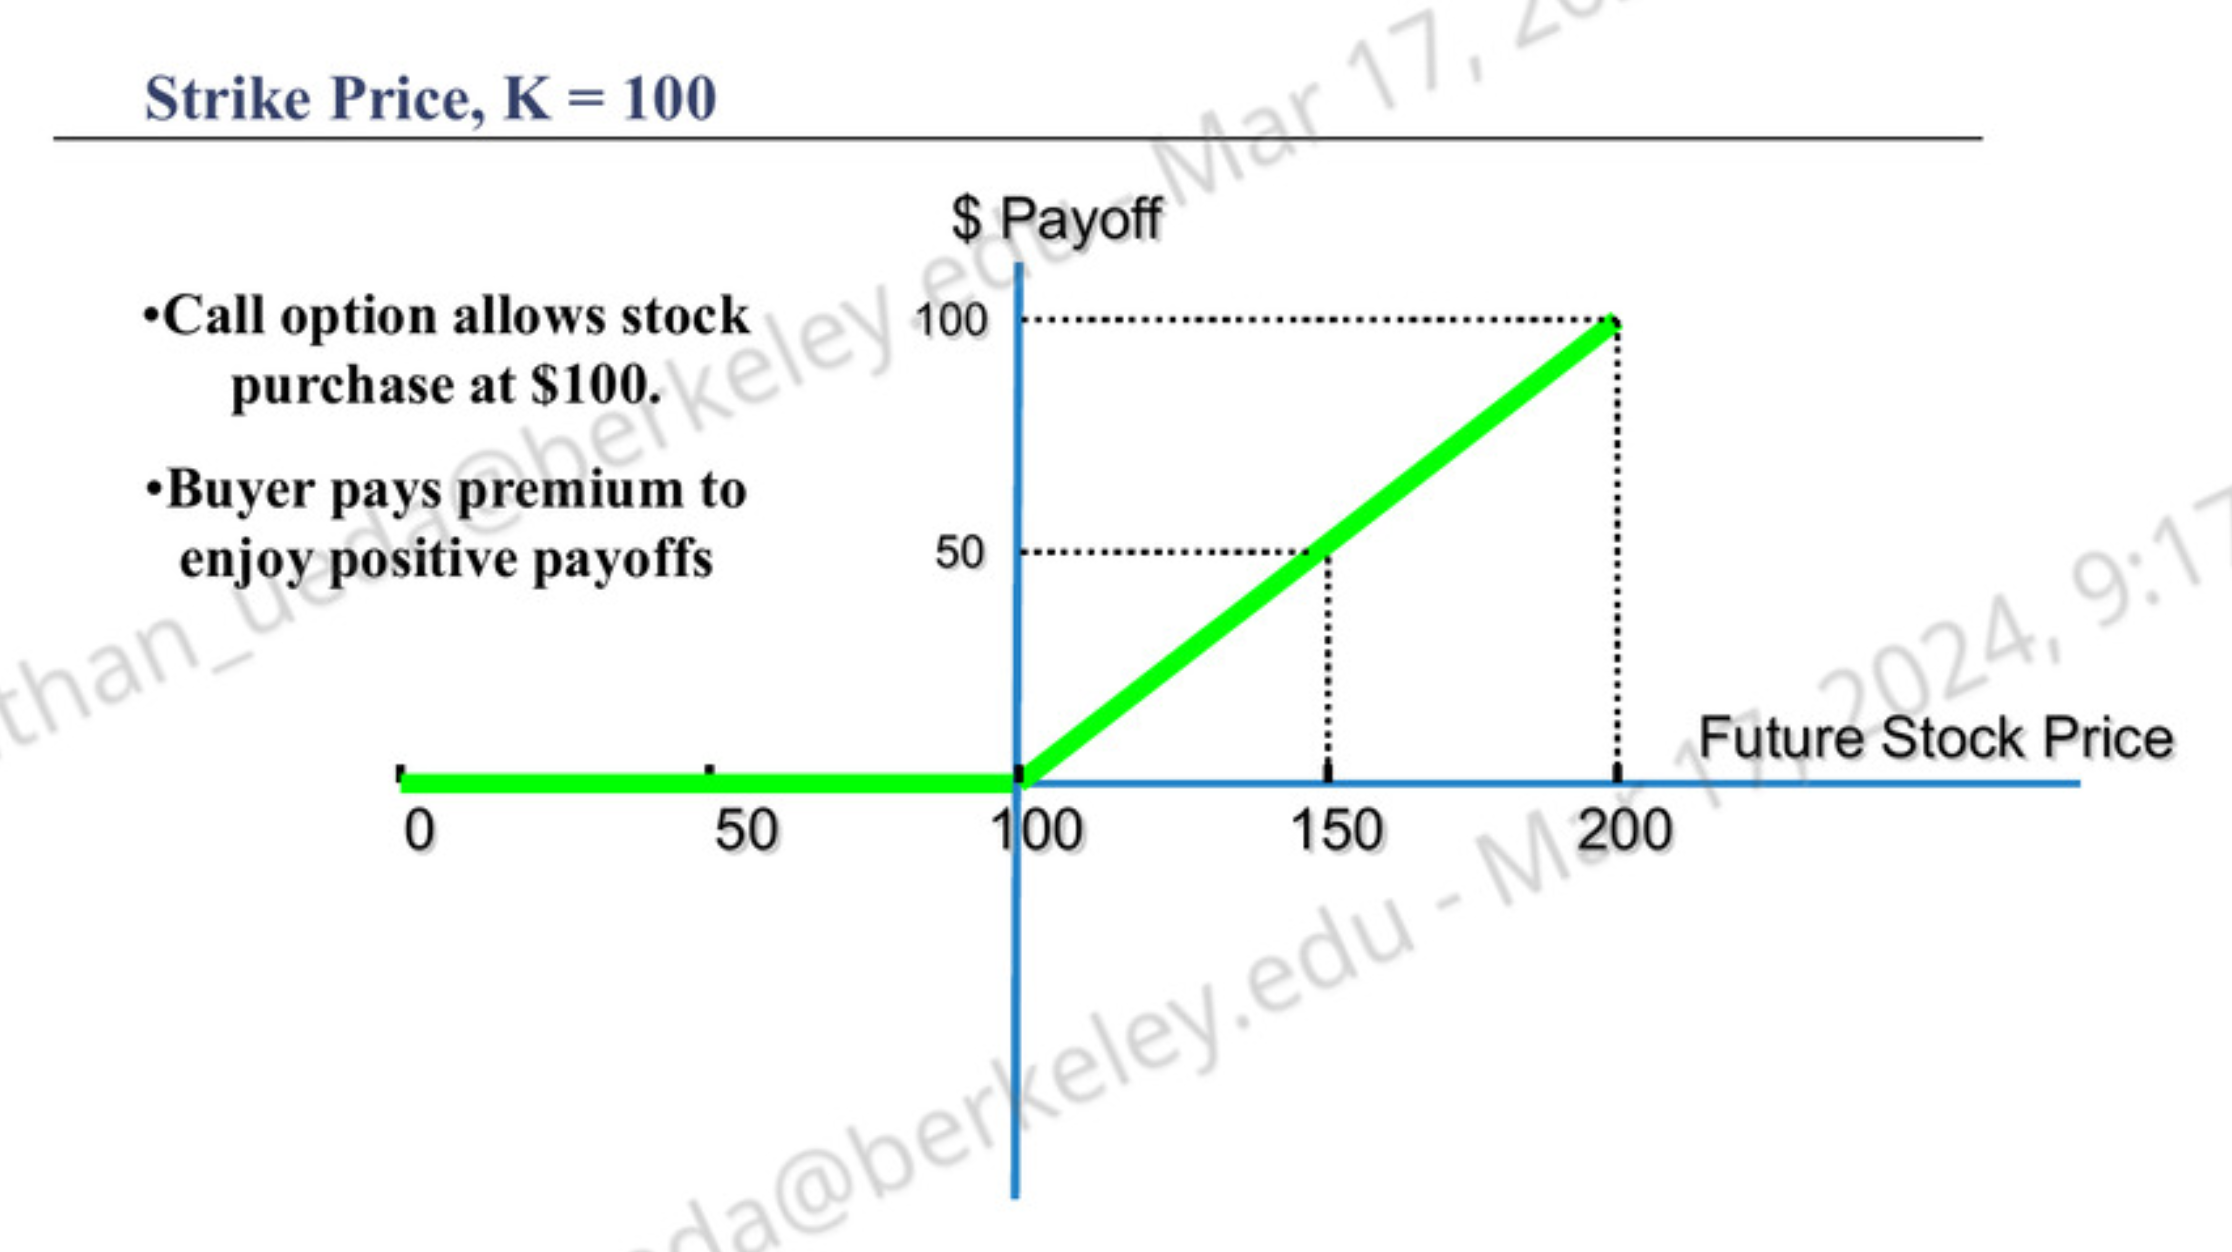
\includegraphics[width=4in]{imgs/call_payoff.png}
    \caption{Call payoff at expiration.}
\end{figure}

\begin{figure}[H] 
    \centering 
    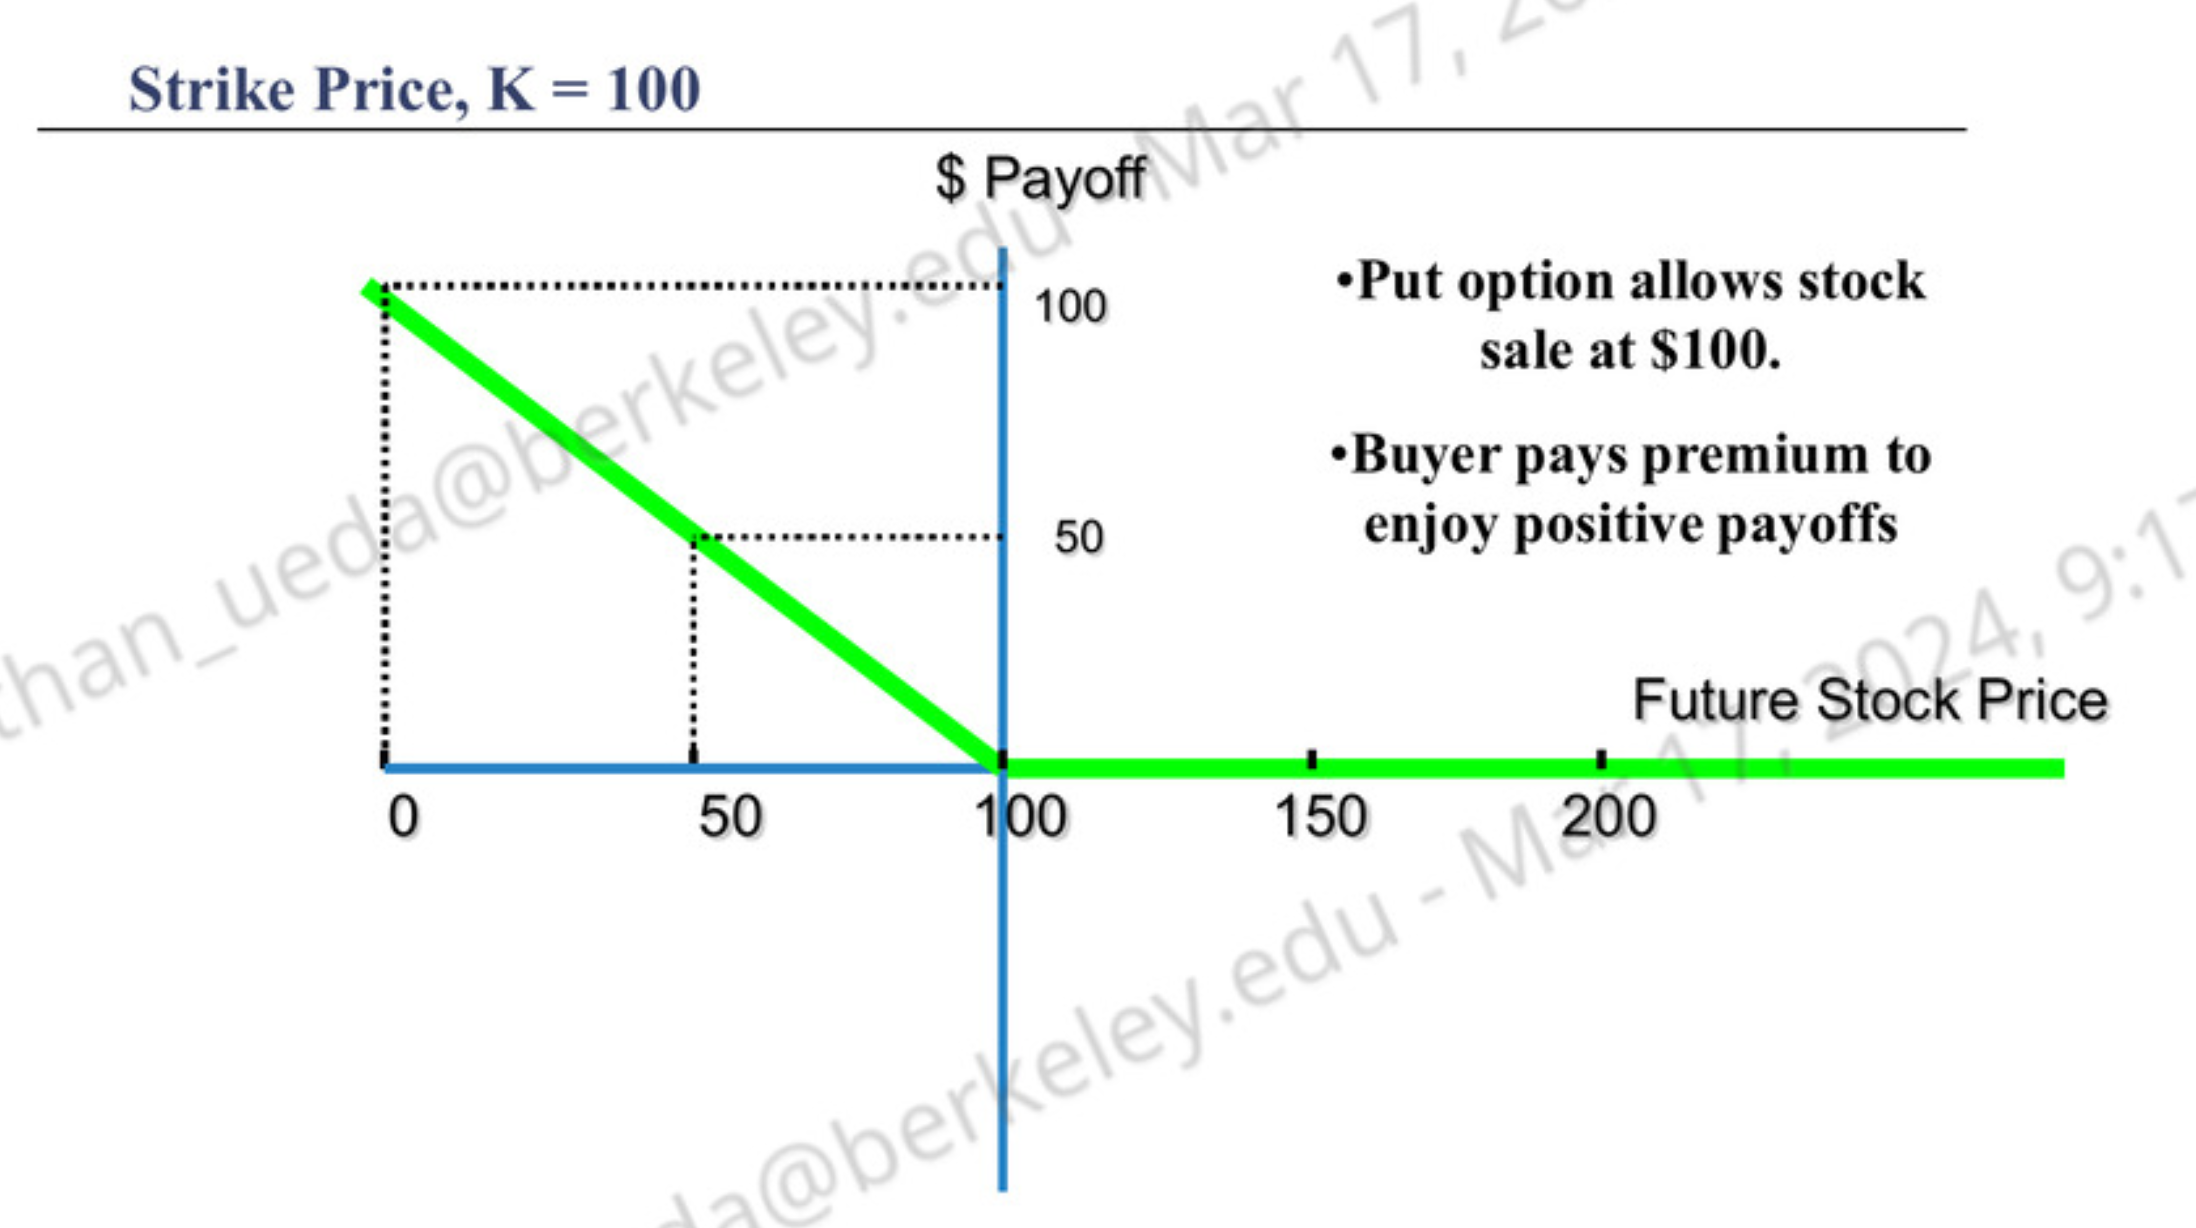
\includegraphics[width=4in]{imgs/put_payoff.png}
    \caption{Put payoff at expiration.}
\end{figure}

\textbf{Formulas for Options Payoffs}
\begin{itemize}
    \item Call: $C = \text{Max}[0, S-K]$
    \item Put: $P = \text{Max}[0, K-S]$
\end{itemize}

\subsubsection{One Period, Two State Binomial Model}
\begin{itemize}
    \item Two points in time: $t=0$ and $t=1$
    \item Two assets: a bond and a stock 
    \item Price of bond at time $t$ is denoted $B_t$
    \item Price of stock at time $t$ is denoted $S_t$
    \item The bond price is deterministic and given by 
    \[B_0 = 1\]
    \[B_1 = R\]
    where $R \ge 1$.
    \item The stock price is a stochastic process where 
    \[S_0 = S\]
    \[
    S_1 = \begin{cases}
        uS, & \text{with probability } p_u \\
        dS, & \text{with probability } p_d
    \end{cases}
    \] where $u \ge d$.

    \begin{figure}[H] 
        \centering 
        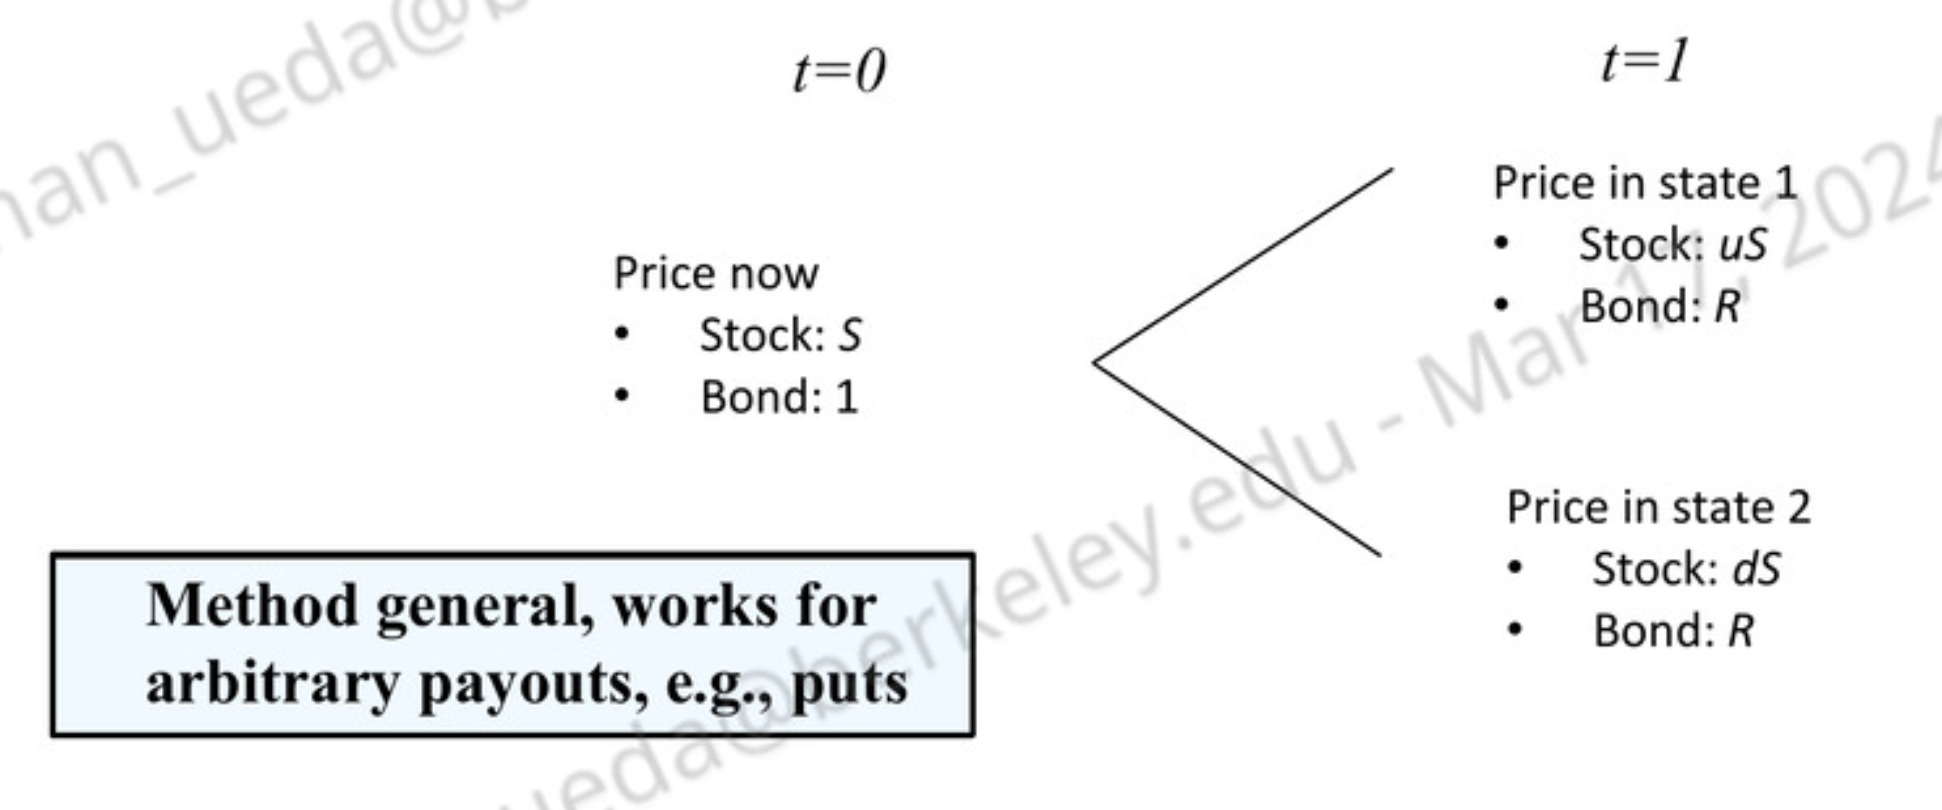
\includegraphics[width=4in]{imgs/one_period_two_state_bin_tree_model.png}
        \caption{Price dynamics}
    \end{figure}
\end{itemize}

\subsubsection{Basic Probability}
\begin{itemize}
    \item Assume sample space $\Omega = \{\omega_1, \ldots, \omega_M\}$
    \item A set of events $\{B_1, \ldots, B_m\}$ forms a \textit{partition} of $\Omega$ if 
    $\cup_i B_i = \Omega$ and $B_i \cap B_j = \emptyset$ when $i \ne j$
    \item Conditional probability is $P(A|B) = \frac{P(A \cap B)}{P(B)}$
    \item For a partition of $\Omega$ $\{B_1, \ldots, B_m\}$, LOTP states that for any event 
    $A$, $P(A)= \sum_i P(A \cap B_i) = \sum_i P(A|B_i)P(B_i)$
    \item Law of iterated expectations states for a r.v. $\tilde{X}$, $E[E[\tilde{X}|B]] = 
    E[\tilde{X}]$. Essentially what this is saying is that the best forcast of the forcast for
    $\tilde{X}$ given $B$ is simply the unconditional expectation of $\tilde{X}$.
    \item Bayes rule states $P(A|B) = \frac{P(B|A)P(A)}{P(B)}$
\end{itemize}

\subsubsection{General $n$ Step Binomial Tree Method}

\begin{itemize}
    \item The general unconditional risk neutral pricing formula for the general $n$ step 
    binomial tree method is 
    \[C(0) = \frac{1}{R^n}\sum_{k=0}^{n} {n \choose k} q^k {(1-q)}^{n-k} C(n,k)\]
    which discounts by $R$ $n$ times, where the are $ {n \choose k} $ total paths to a 
    terminal node, each path having a $q^k {(1-q)}^{n-k}$ is the probability of reaching one 
    of those terminal paths. So $\sum_{k=0}^{n} {n \choose k} q^k {(1-q)}^{n-k}$ get the total 
    probability of reaching the terminal nodes from any of the paths multiplied by $C(n,k)$.
\end{itemize}

\subsection{The General Multi-Period Model}
\begin{itemize}
    \item This model has no restriction on the number of states, the number of assets, and is 
    not restricted to being binomial. 
\end{itemize}

\textbf{Information Revelation in Multi-Period Economies}
\begin{itemize}
    \item Consider the following three period economy with 11 states 
    
    \begin{figure}[H] 
        \centering 
        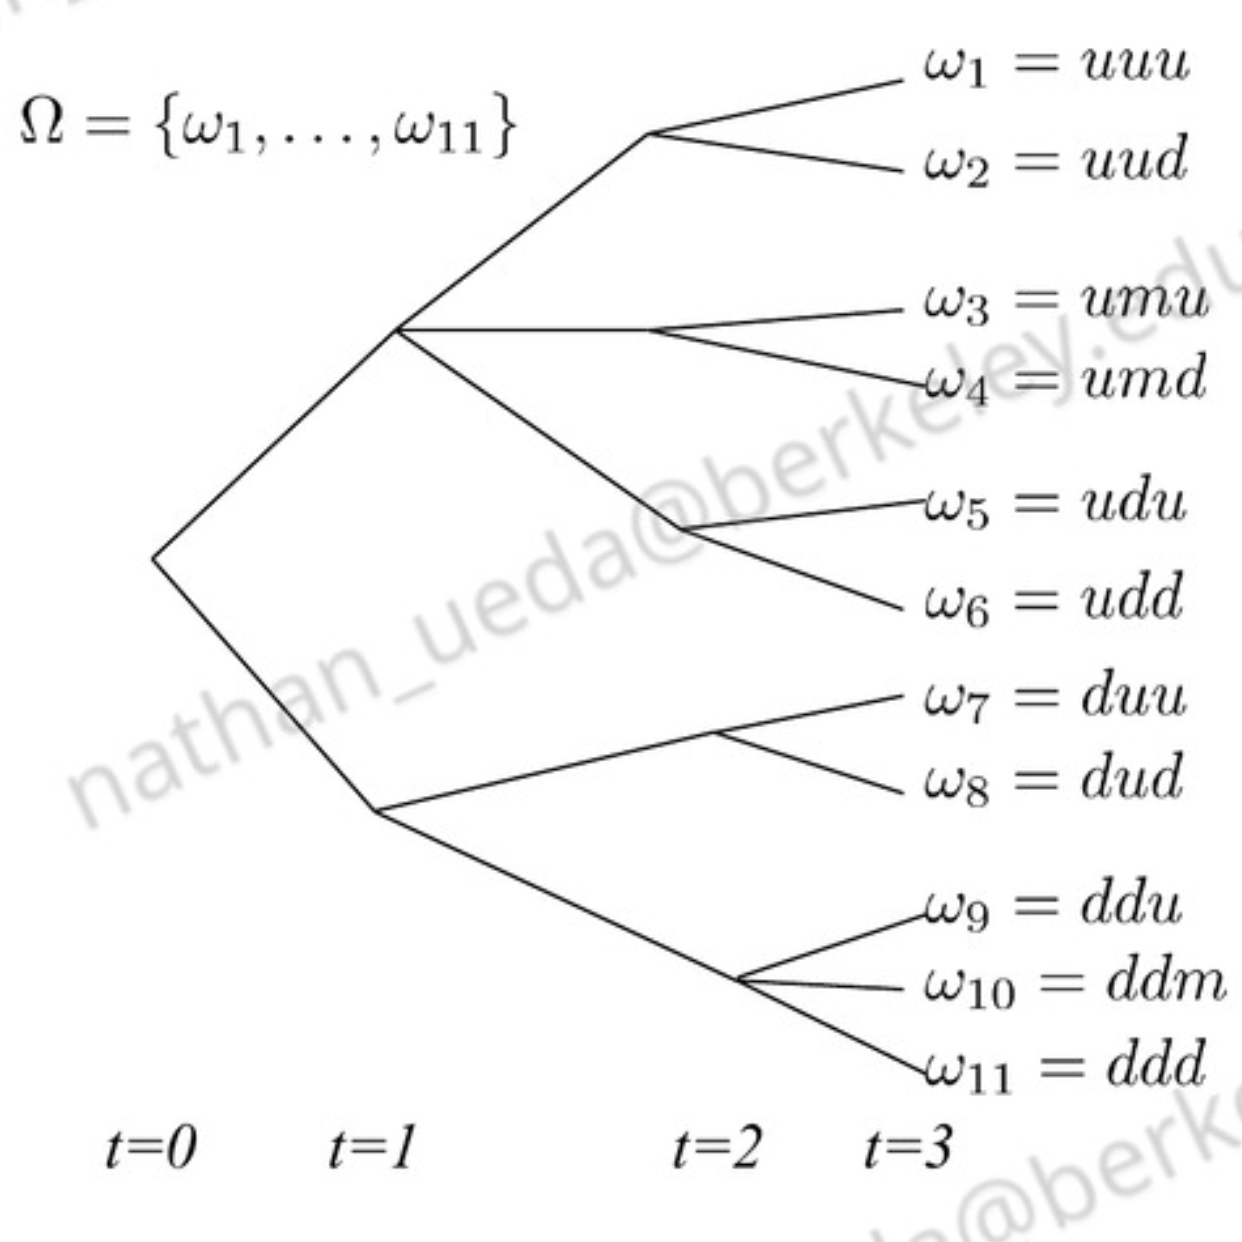
\includegraphics[width=4in]{imgs/three_period_economy.png}
        \caption{11 state, 3 period economy}
    \end{figure}
    
    \item We want to introduce a way to rebalance and have the formulas to keep track of the 
    values dynamics at any point in time.
    \item Naively, a trading strategy is a function of time and the state space 
    \[h:  \{0, \ldots, T\} \times \Omega \rightarrow \mathbb{R}^N\]
    and the strategy must be careful not to allow for taking future (at the time unknown) into 
    account. 
    \item Therefore, in the dynamic setting, we need to define trading strategies so that they 
    only use available information. 

    \begin{figure}[H] 
        \centering 
        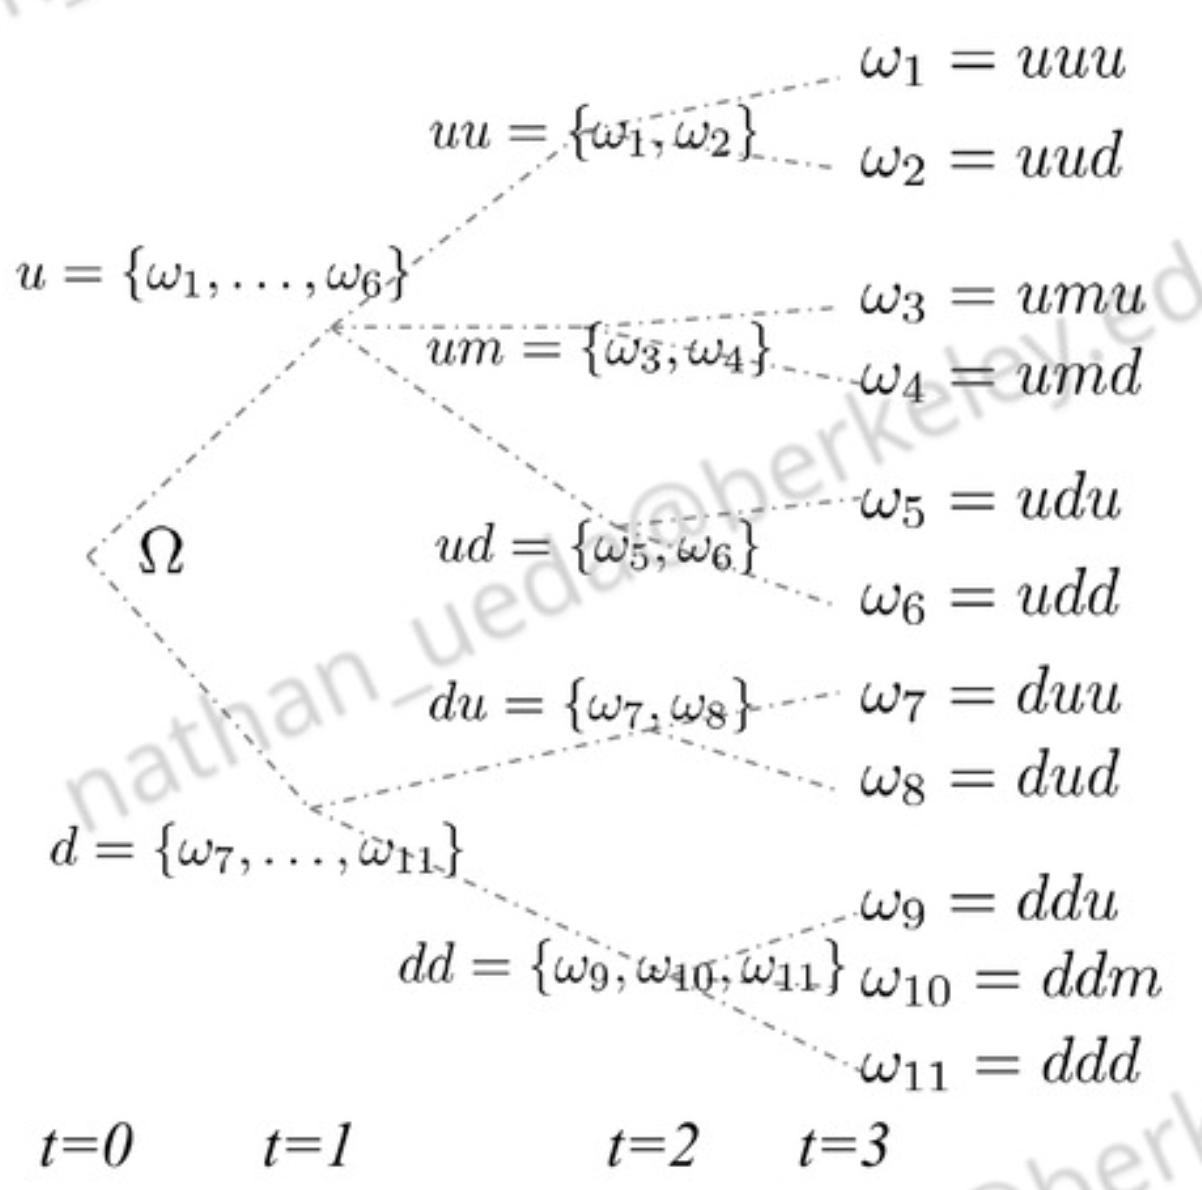
\includegraphics[width=4in]{imgs/three_period_economy_2.png}
        \caption{11 state, 3 period economy, showing }
    \end{figure}

    \item In this economy, we define four $\sigma$-algebras
    \begin{itemize}
        \item $\mathcal{F}_0 = \sigma(\{\Omega\})$
        \item $\mathcal{F}_1 = \sigma(\{u,d\})$
        \item $\mathcal{F}_2 = \sigma(\{uu, um, ud, du, dd\})$
        \item $\mathcal{F}_3 = \sigma(\Omega)$
    \end{itemize}
    \item Note that $\mathcal{F}_0 \subset \mathcal{F}_1 \subset \mathcal{F}_2 \subset 
    \mathcal{F}_3$ 
    \item At $\mathcal{F}_0$ we have no information and at $\mathcal{F}_3$ we have the exact 
    state that occurred. 
    \item A natural interpretation is that $\mathcal{F}_t$ represents how much refined 
    the known information is at time $t$.
    \item A \textit{filtration}, $\underline{\mathcal{F}}$ on the probability space $\Omega, 
    \mathcal{F}, \mathbb{P}$ is an increasing sequence of $\sigma$-algebras, $\mathcal{F}_0 
    \subset \hdots \subset \mathcal{F}_T \subset \mathcal{F}$. As $T$ increases, the $\sigma$-
    algebras becomes more refined since more information is known. 
    \item An $\underline{\mathcal{F}}$-\textit{adapted} (random) process, $X: T \times \Omega 
    \rightarrow \mathbb{R}$, where we, with a slight abuse of notation, write $T=\{0,1,\ldots,
    T\}$, is a process, such that $X_t$ is $\mathcal{F}_t$-measurable for all $t$. 
    Intuitively, this definition takes into account that $X_t$ can only depend on the 
    information that is available at time $t$. If the process is not adapted, then it cheats 
    and uses future information. If it is adapted, it is only using the available information.
    \item An $\underline{\mathcal{F}}$-martingale is an adapted process, $m$, such that for all 
    $0 \le s \le t, E[m_t|\mathcal{F_s}]=m_s$. In other words, the best forecast is not expected 
    to change (the best forecast is what it is right now). It follows immediately from the law 
    of iterated expectations that $Y_t$ defined above is a martingale. 
\end{itemize}

\textbf{The Multiperiod Security Market}
\begin{itemize}
    \item Given a probability space $(\Omega, \mathcal{F}, \mathbb{P})$, a filtration 
    $\underline{\mathcal{F}}=(\mathcal{F}_0, \ldots, \mathcal{F}_T)$, with $\mathcal{F}_0= \{
    \emptyset, \Omega\}$ (i.e. we know nothing) and $\mathcal{F}_T = \sigma(\Omega)$ (i.e. we 
    know everything), and a market with $N$ traded assets.
    \item Each security is a claim to an adapted \textit{dividend process}. Formally, we 
    define the vector valued adapted process as $\delta_t \in \mathbb{R}^N$, where 
    ${(\delta_t)}_i$ represents the dividends paid by asset $i$ at time $t$.
    \item Each security is associated with an adapted \textit{price process}, representing the 
    price of the security, right after the dividend is paid (\textit{ex dividend}). Formally,
    we defined the vector valued adapted process as $\boldsymbol{s}_t \in \mathbb{R}^N$, where 
    ${(\boldsymbol{s}_t)}_i$ represents the price of asset $i$ at time $t$, just after 
    dividends have been paid. 
    \item The before-dividend (\textit{cum dividend}) price proess is $\boldsymbol{s}_t +
    \delta_t$.
    \item The market is summarized by the dividend price pair $(\delta, \boldsymbol{s})$. This 
    pair gives the price and dividend amount for every possible state that may occur. This is 
    the multiperiod version of the $s^0$ and $\boldsymbol{D}$ we had in the single period 
    setting. 
    \item In the multiperiod model, we separate the value we get from dividends and price 
    appreciation. 
    \item A \textit{trading strategy} is a vector valued adapted process $\boldsymbol{h}_t \in 
    \mathbb{R}^N$ where $\boldsymbol{h}_{-1} = 0$. $\boldsymbol{h}_{-1}$ is an artifical time 
    $t=-1$ where we have nothing. The trading strategy can now trade over time. 
    \item The \textit{payoff process} generated by a trading strategy $\delta_t^
    {\boldsymbol{h}} \in \mathbb{R}$ is an adapted process defined by 

    \[
    \delta_t^{\boldsymbol{h}} = \boldsymbol{h}'_{t-1}(\boldsymbol{s}_t + \delta_t) - 
    \boldsymbol{h}'_{t}\boldsymbol{s}_t.
    \]
    that represents how much money the process generates over time. $\boldsymbol{h}'_{t-1}$ is 
    how much of each stock invested at $t-1$ multiplied by $(\boldsymbol{s}_t + \delta_t)$ 
    which is the price of the stock at time $t$ right before the dividend (cum dividend), 
    $\delta_t$, is paid. 
    \item Put simply, $\boldsymbol{h}'_{t-1}(\boldsymbol{s}_t + \delta_t)$ is the value of our 
    portfolio cum-dividend based on how we invested at time $t-1$ and $\boldsymbol{h}'_{t}
    \boldsymbol{s}_t$ is the value of the portfolio after we rebalanced the portfolio, at time 
    $t$, and their difference is the amount we get through the rebalancing. 
    \item In the case of assets that do not pay dividends, this reduces to  
    \[
    \delta_t^{\boldsymbol{h}} = (\boldsymbol{h}_{t-1}-\boldsymbol{h}_{t})'\boldsymbol{s}_t
    = -(\boldsymbol{h}_{t} + \boldsymbol{h}_{t-1}) = -(\Delta \boldsymbol{h}\_{t})'
    \boldsymbol{s}_t
    \]   
    \item The \textit{value process} of a trading strategy is $V_t^{\boldsymbol{h}} = 
    \boldsymbol{h}'_{t}\boldsymbol{s}_t$.
    \item Given, an adapted \textit{consumption process} (which is a plan for how much we plan 
    to comsume), $c_t$, a trading strategy is said to be \textit{self-financed} if 
    $\delta_t^{\boldsymbol{h}} = c_t$ for $t=1, \ldots, T$. In other words, a trading strategy 
    is self-financed if we set up the consumption process so that we get exactly the same 
    payoff process, $\delta_t^{\boldsymbol{h}}$ as you wish to consume, $c_t$. 
    \item We mainly focus on the cases where we are not consuming anything, that is $c_t=0$. 
    \item The below figure justifies the formula for the payoff process cum dividend
    \begin{figure}[H] 
        \centering 
        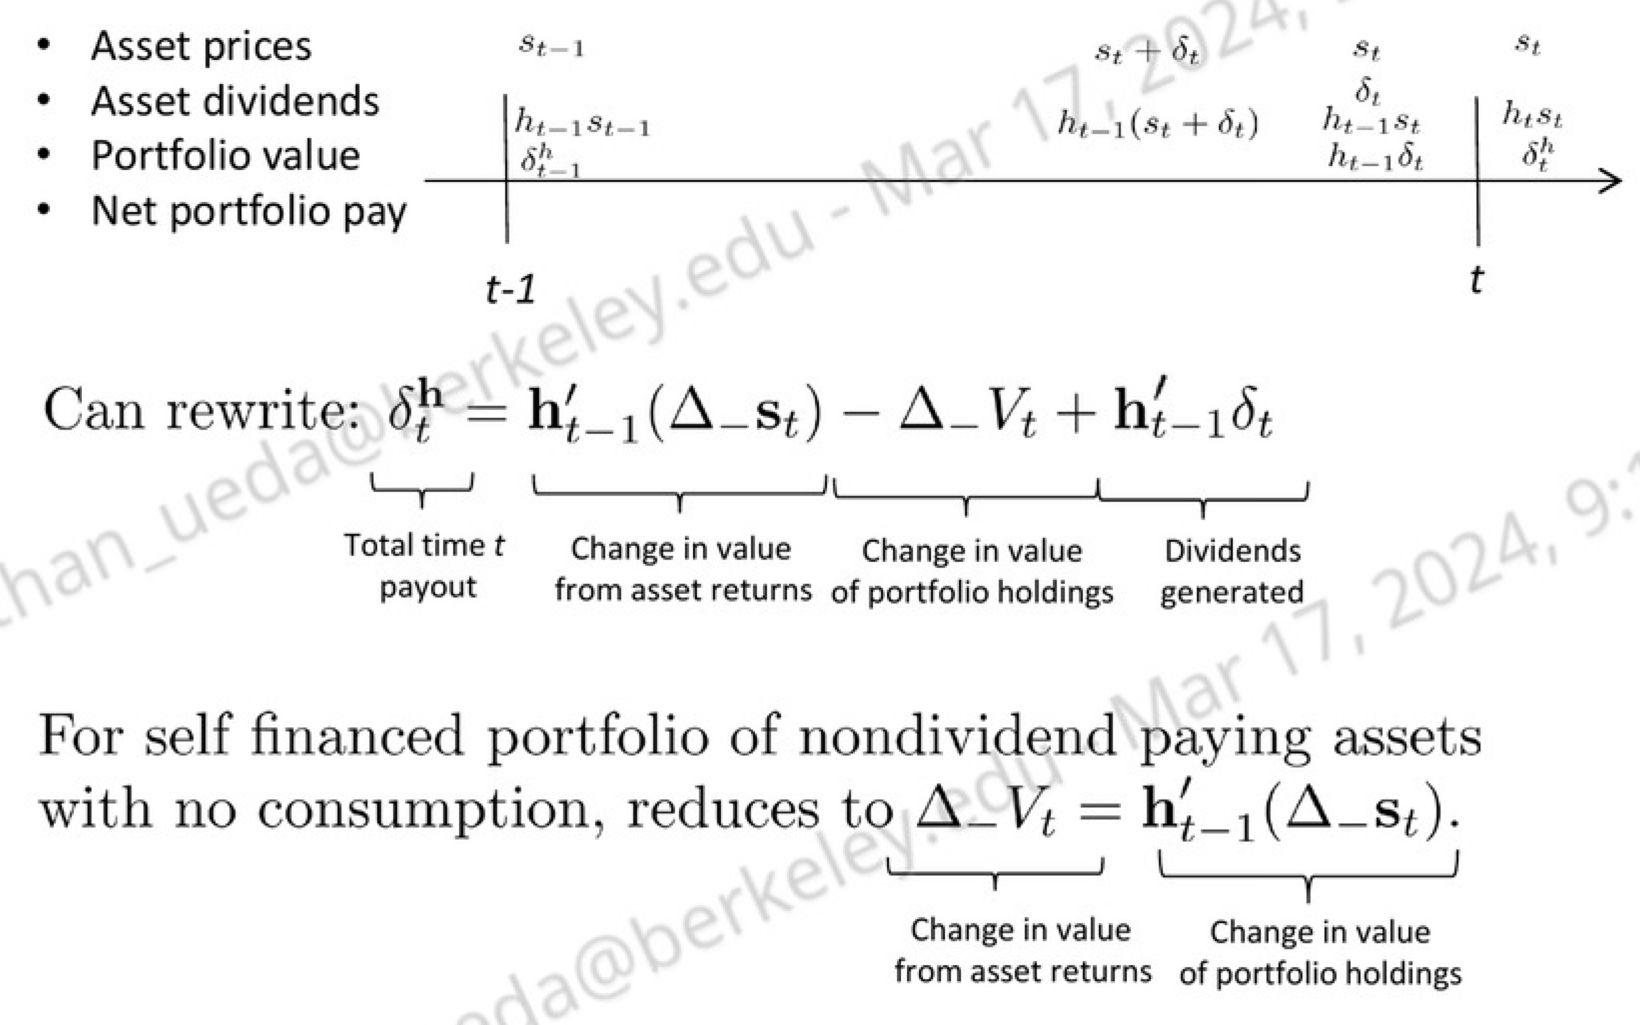
\includegraphics[width=5in]{imgs/payoff_process_cum_div_justified.jpeg}
        \caption{At time $t-1$, we just received our dividend payment so the porfolio value is 
        currently $\boldsymbol{h}'_{t-1} \boldsymbol{s}_{t-1}$. Next, we have the cum dividend 
        price process. Next, dividends are paid, in the amount $\boldsymbol{h}_{t-1}\delta_t$, 
        which can then be reinvested into the portfolio $\boldsymbol{h}_{t}$, the rebalanced 
        portfolio.}
    \end{figure}

    \item Deriving the new rewritten formula  
    \begin{align*}
        \delta_t^{\boldsymbol{h}} 
        &= \boldsymbol{h}'_{t-1}(\Delta\_\boldsymbol{s}_t) - \Delta \_ V_t + 
        \boldsymbol{h}'_{t-1} \delta_t \\
        &= \boldsymbol{h}'_{t-1}(\boldsymbol{s}_t - \boldsymbol{s}_{t-1}) - 
        (\boldsymbol{h}'_{t}\boldsymbol{s}_{t} - \boldsymbol{h}'_{t-1}\boldsymbol{s}_{t-1}) + 
        \boldsymbol{h}'_{t-1} \delta_t \\
        &= \boldsymbol{h}'_{t-1}\boldsymbol{s}_t - \boldsymbol{h}'_{t-1}\boldsymbol{s}_{t-1} - 
        \boldsymbol{h}'_{t}\boldsymbol{s}_{t} + \boldsymbol{h}'_{t-1}\boldsymbol{s}_{t-1} + 
        \boldsymbol{h}'_{t-1} \delta_t \\
        &= \boldsymbol{h}'_{t-1}\boldsymbol{s}_t - \boldsymbol{h}'_{t}\boldsymbol{s}_{t} + 
        \boldsymbol{h}'_{t-1} \delta_t \\
        \delta_t^{\boldsymbol{h}} &= \boldsymbol{h}'_{t-1}(\boldsymbol{s}_t + \delta_t) - 
        \boldsymbol{h}'_{t}\boldsymbol{s}_t
    \end{align*}
    
    \begin{figure}[H] 
        \centering 
        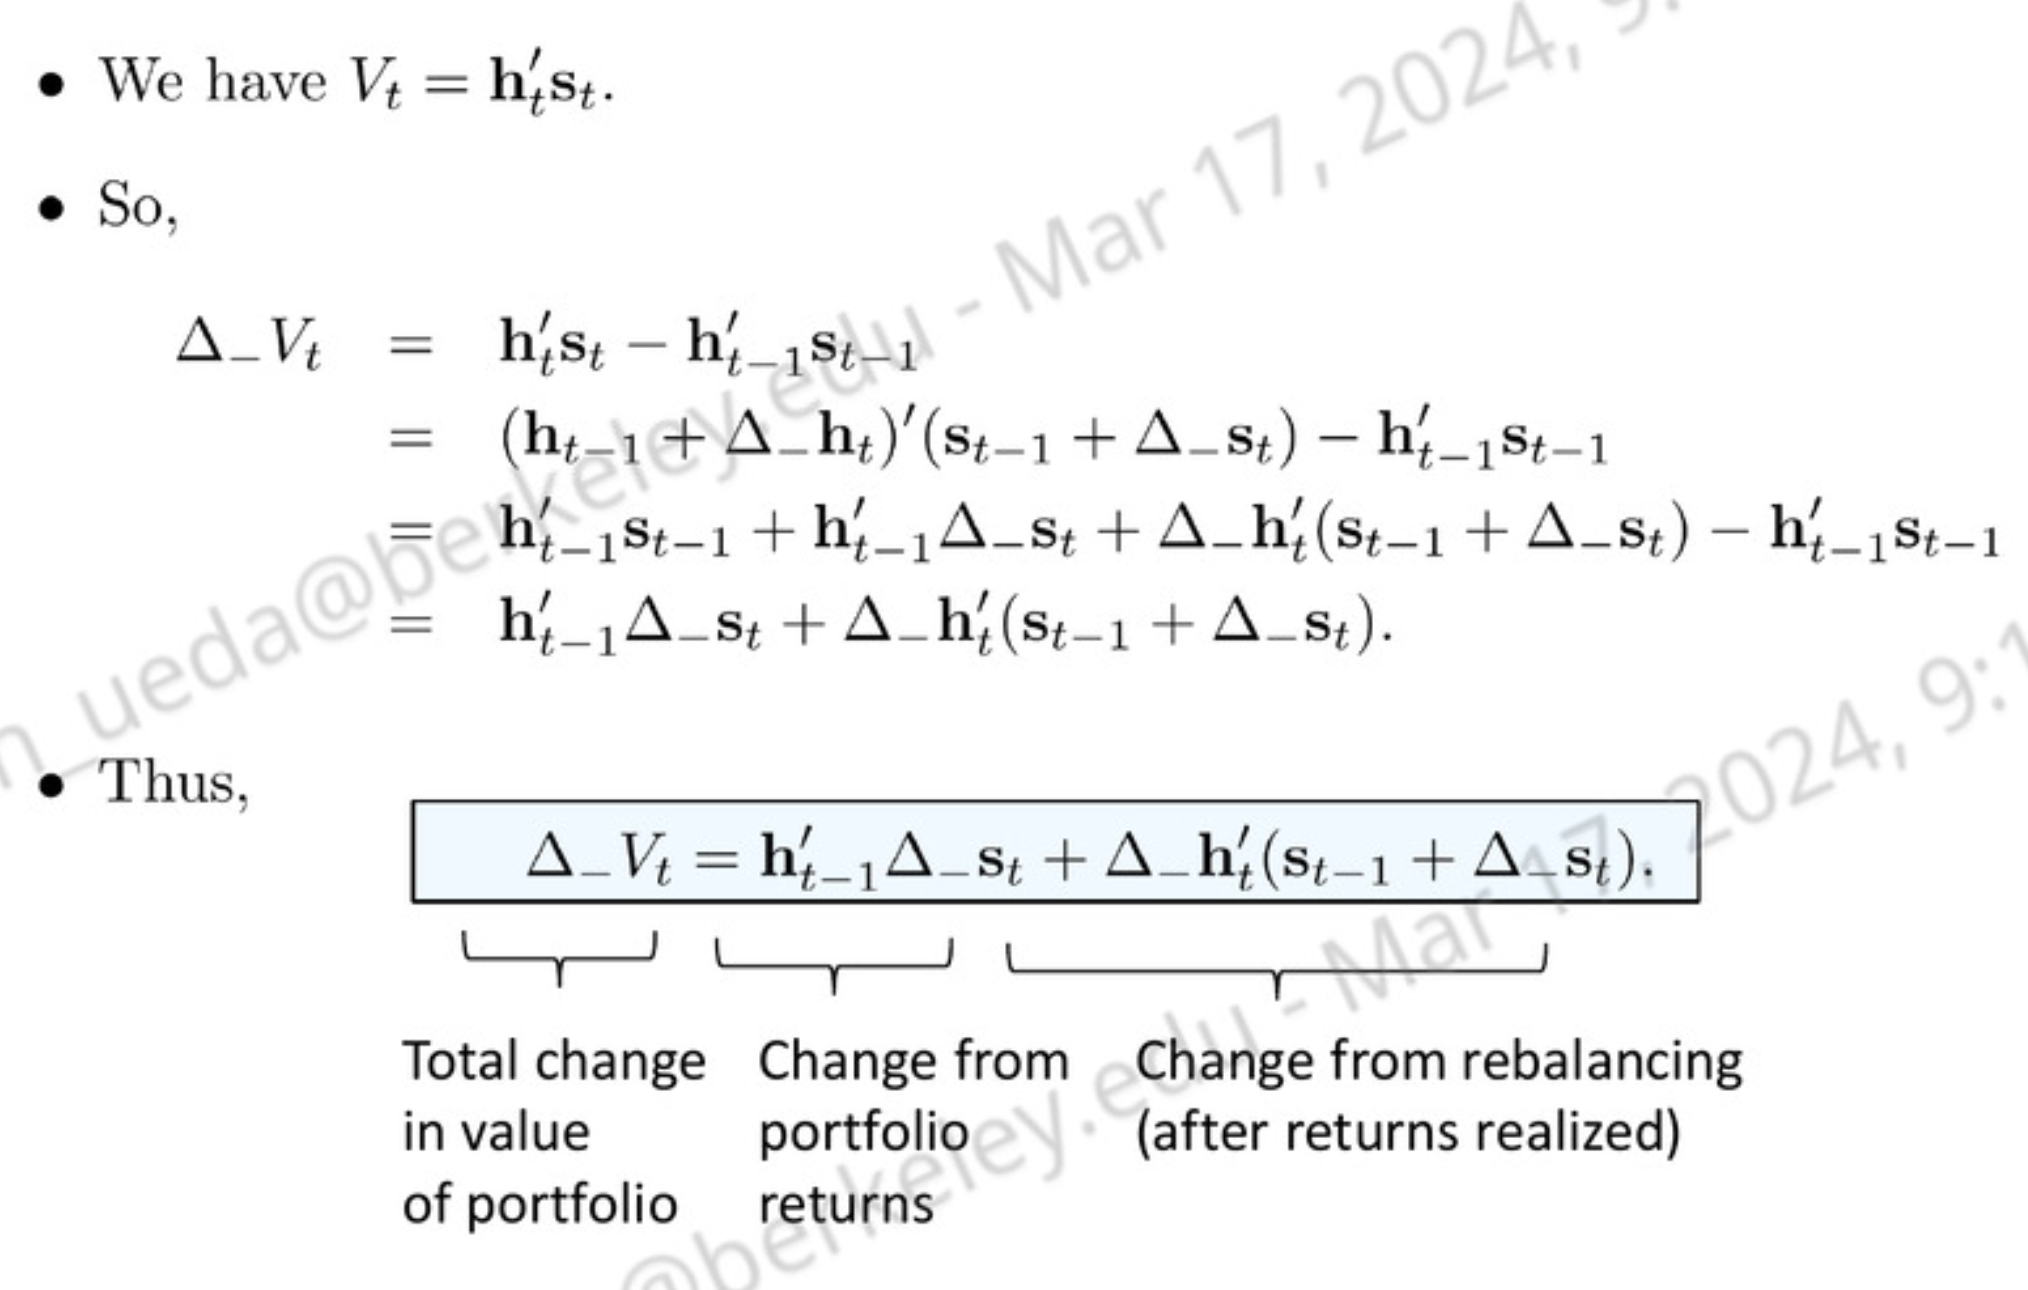
\includegraphics[width=5in]{imgs/change_in_value_process.png}
        \caption{Denotes the change in the value of the portfolio. Has relevance to Ito's 
        formula in a much simpler manner.}
    \end{figure}
    
    \item A trading strategy, $\boldsymbol{h}$, provides an arbitrage if $\delta_t^
    {\boldsymbol{h}} \ge 0$ for all $t$, for all $\omega \in \Omega$ (no negative cash flows 
    anywhere), and $\delta_t^{\boldsymbol{h}} > 0$ for some $t$ and $\omega \in \Omega$ (a 
    strictly positive cash flow somewhere), and $\boldsymbol{h}_T = 0$ (must liquidate entire 
    portfolio).
    
    \item Define $\bar{L}$, the (augmented) space of 
    adapted processes, $\Theta$, the space of trading strategies, $\Theta = \{\boldsymbol{h}:
    \boldsymbol{h} \text{ is a trading strategy}\}$, and $\mathcal{\bar{R}}$, the augmented 
    marketed (reachable) space, $\mathcal{\bar{R}} = \{\delta^{\boldsymbol{h}} : 
    \boldsymbol{h} \in \Theta\}$ (all the different possible payouts that are adaptaive at any 
    point in time in any state). Then we have the natural embedding:
    \[\mathcal{\bar{R}} \subset \bar{L} \subset \mathbb{R}^{T \times \Omega} \]
    where $\mathbb{R}^{T \times \Omega}$ is all states at any point in time, regardless of
    being adaptive. 
    
    \item Similarly, we define the space of adapted processes from $t=1, \ldots, T, L = \{l_t :
    \{1, \ldots, T\} \times \Omega \rightarrow \mathbb{R} : l_t = y_t, \; t = 1, \ldots, T, 
    \text{ for some } y \in \bar{L}\}$ and the marketed space $\mathcal{R} = \{m_t : \{1, 
    \ldots, T\} \times \Omega \rightarrow \mathbb{R} : m_t = y_t, \; t = 1, \ldots, T, \text{
    for some } y \in \mathcal{\bar{R}}\}$ with the natural embedding 
    \[\mathcal{R} \subset L \subset \mathbb{R}^{(T-1) \times \Omega}\]
    
    \item The relation of $\mathcal{R}$ to $\mathcal{\bar{R}}$ is the same as in the single 
    period binomial model, that is, $\mathcal{R}$ does not take into account time $t=0$ cash 
    flows while $\mathcal{\bar{R}}$ does. 

    \item The reachable payoff space is the different types of payoffs we can generate by 
    having an adaptive trading strategy. 

    \item The market is said to be complete if $\mathcal{R} = L$.
    
    \item A \textit{stochastic discount factor} (the prices today as a function of future 
    prices), $M_t$, is a strictly positive adaptive process, such that for all assets, $i$, 
    \[ 
    {(s_t)}_i = \frac{1}{M_t} E_{\mathbb{P}}^t \left[ \sum_{k=t+1}^{T} M_k {(\delta_k)}_i + 
    M_T {(\boldsymbol{s}_T)}_i\right], \; t < T \]
    
    \item Assume a short term risk free asset: For all $t<T$, for all states $B_t^K$, there is 
    a trading strategy $\boldsymbol{h}$, which invests 1 at $t$ and receives $R_t^k$ ad $t+1$. 
    This defines an adapted \textit{short term process}
    \[R_t = 1 + r_t\]

    \item The $n$-period compounded discount rate is 
    \[R_{t, t+n} = R_t R_{t+1} , \ldots, R_{t+n-1}\]

    showing that the risk free rate may change at each period. 
    
    \item An \textit{equivalent martingale measure} $\mathbb{Q}$ satisfies 
    \[
    {(\boldsymbol{s}_t)}_i = E_{\mathbb{Q}}^t \left[ \sum_{k=t+1}^{T} \frac{{(\delta_k)}_i}
    {R_{t,t+k}} + \frac{{(\boldsymbol{s}_T)}_i}{R_{t,T}}\right], \; t < T
    \]
\end{itemize}

\begin{figure}[H] 
    \centering 
    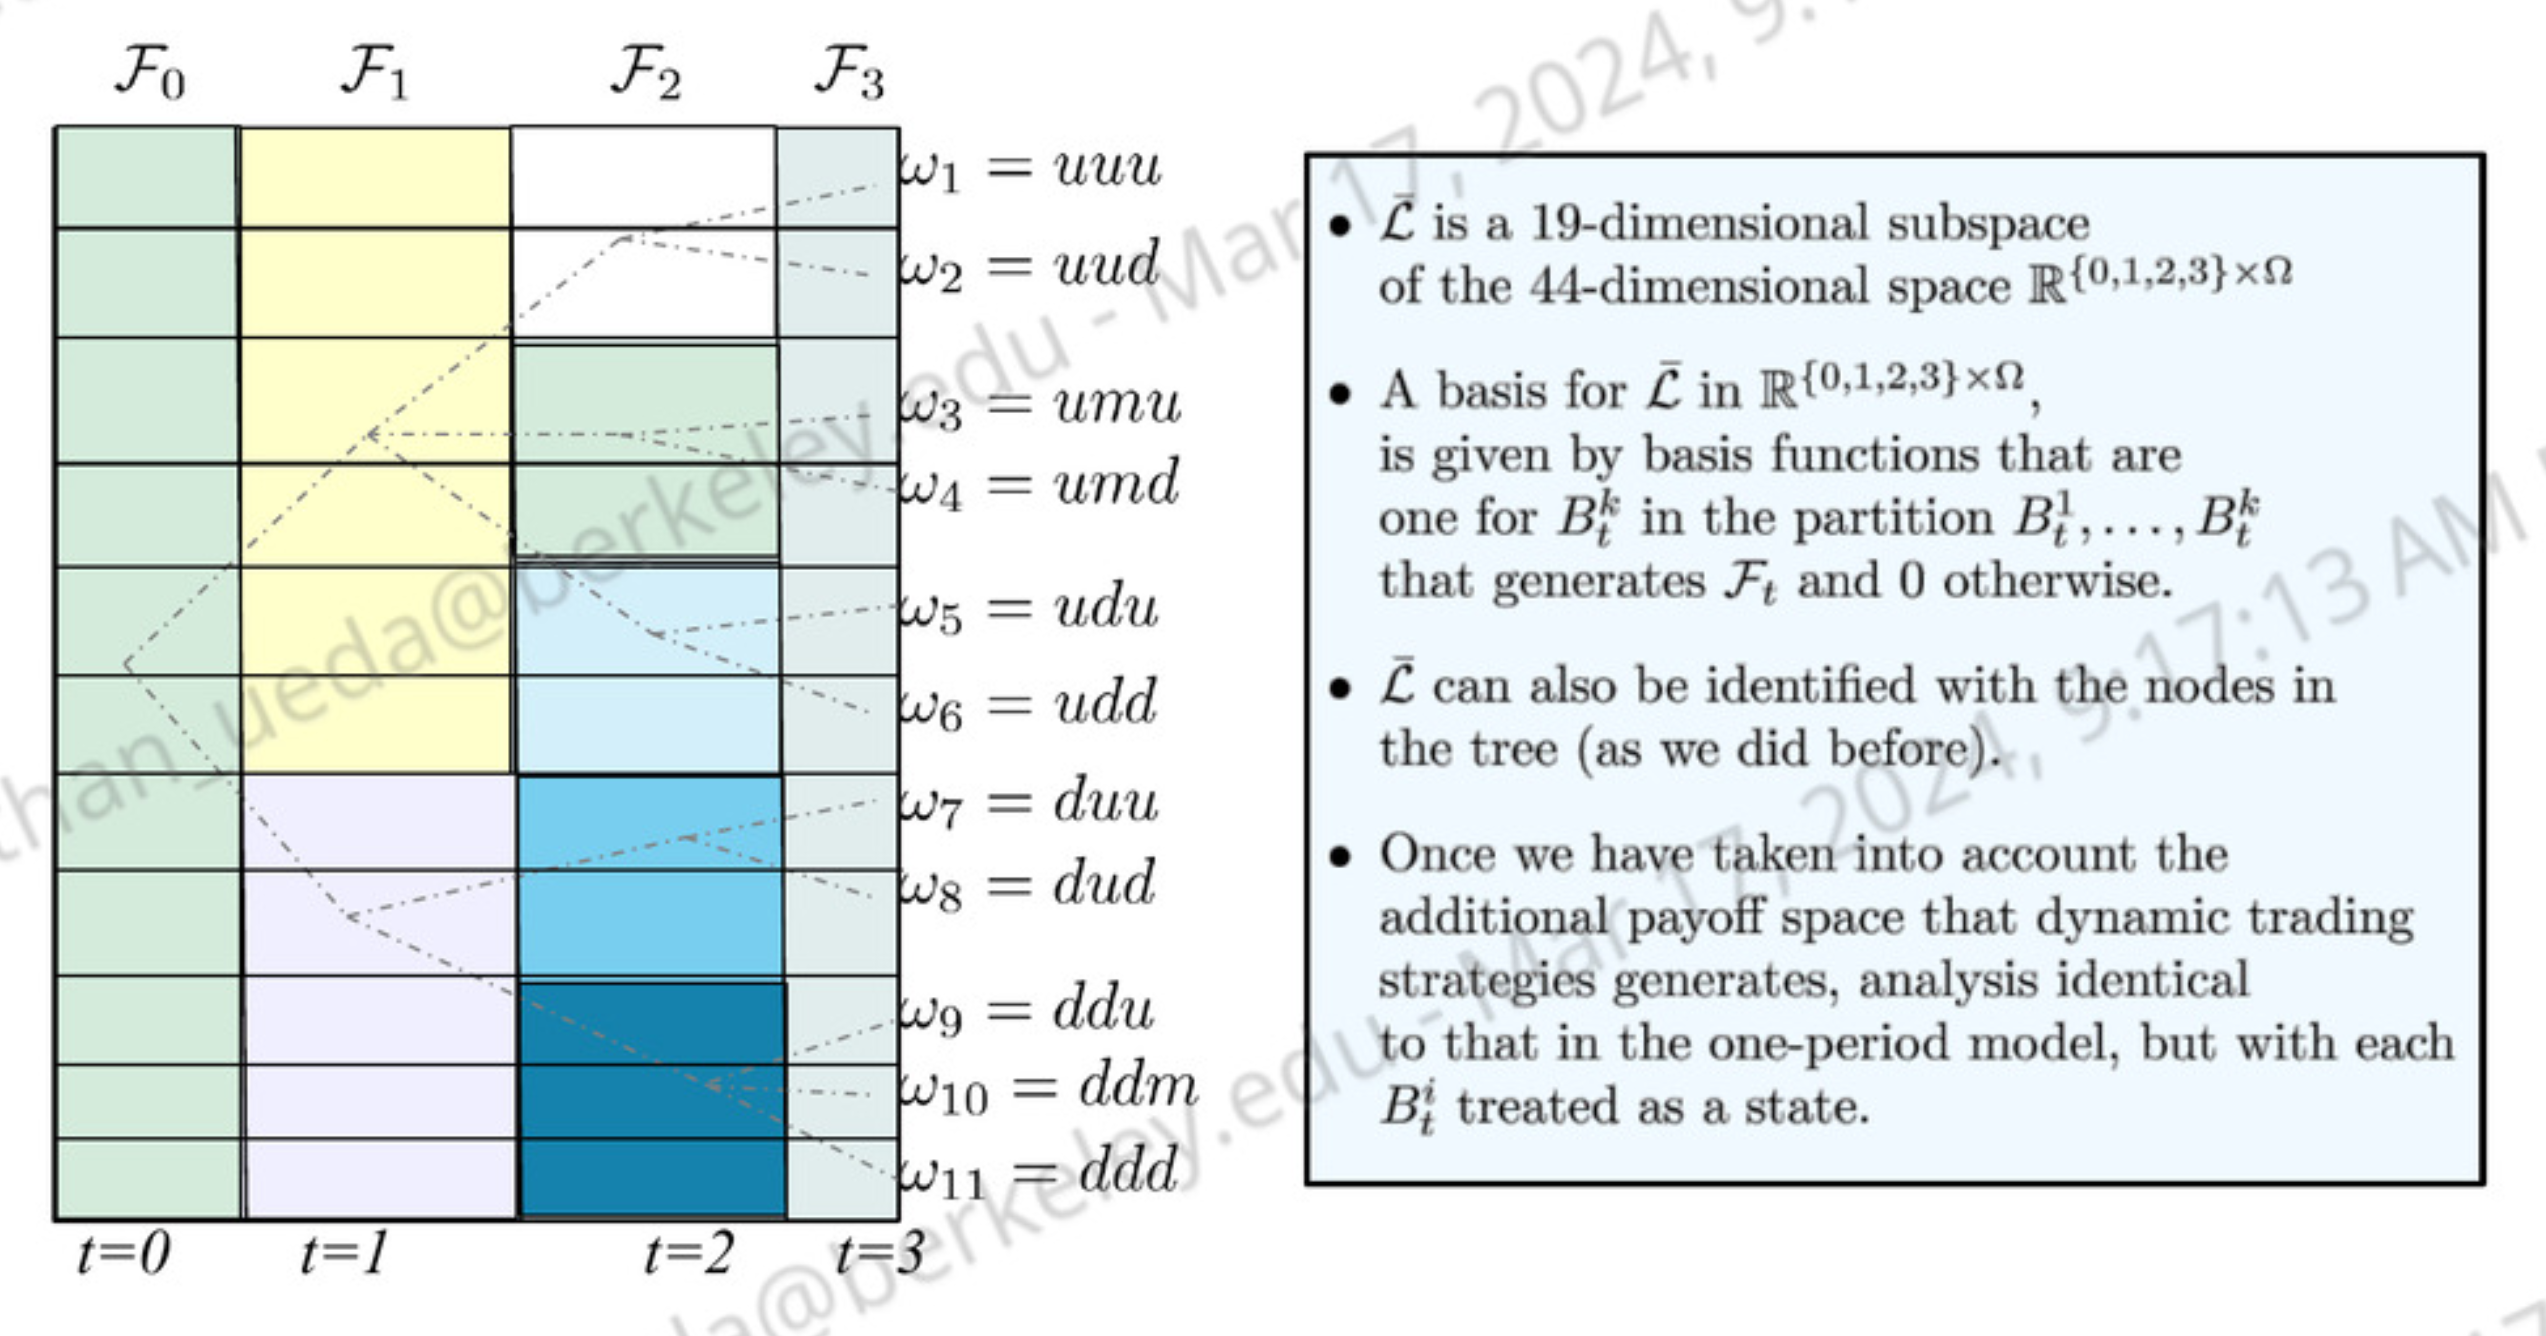
\includegraphics[width=6in]{imgs/embedding.png}
    \caption{The augmented payoff space is 19 dimensional}
\end{figure}

\subsubsection{Multiperiod Fundamental Theorems}
\begin{itemize}
    \item First fundamental theorem: The market admits no arbitrage if and only if there is a 
    stochastic discount factor. 
    \item First fundamental theorem: The market admits no arbitrage if and only if there is an 
    equivalent martingale measure. 
    \item Second fundamental theorem: Given a market that admits no arbitrage. Then the market
    is complete if and only if the equivalent martingale measure is unique.
\end{itemize}

\section{Continuous Time Models}

\begin{itemize}
    \item The motivation for introducing the continuous time model is because it will be very 
    useful in deriving nice solutions and being able to analyze problems in a very tractable 
    manner. 
    \item In the continuous time space, we unfortunately have to give up the partition 
    representation of the sigma algebra (how information is incorporated into the market over 
    time). The reason being is because with a partition we need something where there is a 
    smallest piece of information, but in a continuous time, there is no smallest since they
    can be arbitrarily small. 
    \item A filtration in the continuous space is a nondecreasing family of $\sigma$-algebras,
    $\{\mathcal{F}_t\}, \, \mathcal{F}_s \subset \mathcal{F}_t, \, s < t$, such that 
    $\mathcal{F}_t \subset \mathcal{F}$ for all $t$.
    \item In the same way it is in the discrete model, a stochastic process is adapted if 
    $X_t$ is $\mathcal{F}_t$-measurable for all $t$.
    \item A stochastic process is a martingale if for all $s<t, \; E[X_t|\mathcal{F}_s]=X_s$.
    This means the same thing as it did in the discrete time setting, namely, that its 
    expected value at any future time is whatever its value currently is.  Note that 
    conditioning on $\mathcal{F}_s$ just means that we are conditioning on all the information 
    available at time $s$.
\end{itemize}

\subsection{Brownian Motion}
\begin{itemize}
    \item Brownian motion is a physical phenomenon in which some quantity if constantly 
    undergoing small, random fluctuations. 
    \item A stochastic process, $W_t, \, t \ge 0$ is said to be a \textit{standard Brownian 
    motion} (a Wiener process), if it satisfies the following four properties: 
    \begin{enumerate}
        \item It starts at the origin: $W_0 = 0$
        \item It is normally distributed  $\sim N(0,t)$ and the increment for all $s<t$ is 
        also normally distributed, that is, $W_t - W-s \sim N(0, t-s)$. 
        \item It has independent increments: for all $r<s \le t<u, \, W_u - W_t$ is 
        independent of $W_s - W_r$. This means that whatever happens between $W_s$ and $W_r$ 
        has no effect on what happens between $W_t$ and $W_u$.
        \item It has continuous sample paths: $W_t$ is a continuous function of $t$.
    \end{enumerate}
    \item Clearly, a Wiener process is a martingale process (has not drift, the expected 
    value given all prior information is always the mean, which is 0). 
    \item A \textit{Brownian motion} is a stochastic process, $X_t = X_0 + \mu t + \sigma W_t$
    where $\mu$ and $\sigma > 0$ are constants, and $W_t$ is a standardized Brownian motion. 
    This unstandardized version of Brownian motion allows us to add some drift, $\mu t$, some 
    scaling of the volatility, and some initial starting point, $X_t$.
    \item A \textit{geometric Brownian motion} (GBM) is a stochastic process, $Y_t = e^{X_t}$, 
    where $X_t$ is a Brownian motion. This is what we get when we take $e$ to the power of a 
    Brownian motion, $X_t$, giving it a log normal distribution.
    \item Brownian motions are continuous, but not very smooth and almost surely nowhere 
    differentiable. 
\end{itemize}

\subsection{Multivariate Brownian Motion}
\begin{itemize}
    \item Given $k$-vector of independent standard Brownian motions, $\boldsymbol{W}_t = 
    \begin{bmatrix} W_t^1 \\ \vdots \\ W_t^k \end{bmatrix}$ and vectors $\mu \in \mathbb{R}^k$,
    and $\Sigma = \sigma \sigma^T$, where $\sigma \in \mathbb{R}^{k \times k}$ is invertible
    \begin{itemize}
        \item The process $\boldsymbol{Z}_t = \boldsymbol{Z}_0 + \mu t + \sigma 
        \boldsymbol{W}_t$ is a $k$-dimensional Brownian motion. 
        \item $\boldsymbol{Z}_t \sim N (\mu t, \Sigma t)$, where $\Sigma = \sigma \sigma^T$.
        \item The process $\boldsymbol{Y}_t = \begin{bmatrix} Y_t^1 \\ \vdots \\ Y_t^k 
        \end{bmatrix}$, where $Y_t^i = e^{{(\boldsymbol{Z}_t)}_i}$ is a $k$-dimensional 
        geometric Brownian motion. 
    \end{itemize}
\end{itemize}

\subsection{Continuous Time Trading}
\begin{itemize}
    \item Here we look at how to define continuous time trading between $t=0$ and $t=T$.
    \item We start with the discrete formula for a self financed (this is when consumption 
    equals payoff, that is, $\delta_t^{\boldsymbol{h}} = c_t$ ) portfolio
    \[ \delta_t^{\boldsymbol{h}} = c_t = \boldsymbol{h}'_{t-1}(\Delta\_\boldsymbol{s}_t) - 
    \Delta \_ V_t + \boldsymbol{h}'_{t-1} \delta_t \]
    \item if we have no dividends, we can derive the following
    \begin{align*}
        c_t &= \boldsymbol{h}'_{t-1}(\Delta\_\boldsymbol{s}_t) - \Delta \_ V_t + 
        \boldsymbol{h}'_{t-1} \delta_t \\
        c_t &= \boldsymbol{h}'_{t-1}(\Delta\_\boldsymbol{s}_t) - \Delta \_ V_t \\
        \Delta \_ V_t &= \boldsymbol{h}'_{t-1}(\Delta\_\boldsymbol{s}_t) - c_t
    \end{align*}
    \item Now, we divide $[0,T]$ into $n$ sub periods of length $\Delta t = \frac{T}{n}$.
    \item Therefore, consumption at time $k \Delta t =  c_k \Delta t$, which is talking about 
    consumption per unit of time (i.e. driving 60 mph).
    \item We then rewrite
    \begin{align*}
        \Delta \_ V_t &= \boldsymbol{h}'_{t-1}(\Delta\_\boldsymbol{s}_t) - c_t \\
        \Delta \_ V_{k \Delta t} &= \boldsymbol{h}'_{(k-1)\Delta t}\Delta\_
        \boldsymbol{s}_{k \Delta t} - c_{k \Delta t} \Delta t \\
    \end{align*}
    \item Although we can theoretically sum the differences to get the change in portfolio 
    value 
    \[ 
    V_T - V_0 = \sum_{k=1}^{n}\Delta \_ V_{k\Delta t}
    = \sum_{k=1}^{n}\boldsymbol{h}'_{(k-1)\Delta t} \Delta \_ s_{k \Delta t} - 
    \sum_{k=1}^{n} c_{k \Delta t} \Delta t
    \]
    We prefer to take limits, $\Delta t \rightarrow 0$ and rewrite as 
    \[
    V_T - V_0 = \int_{t=0}^{T}\, dV_t 
    = \int_{t=0}^{T}\boldsymbol{h}'_t \, d\boldsymbol{s}_t - \int_{t=0}^{T} c_t \, dt
    \]
    \item Therefore, we have 2 terms we needs to be able to take the limit of.
\end{itemize}

\begin{itemize}
    \item Consider a simple model with two assets: a standard Brownian motion stock price,
    $S$, and a bond with constant price, $B$ (interest rate is zero and therefore always has 
    the value 1), and a time step $\Delta t$.
    \item $S_{k \Delta t}$ are the values of the standard Brownian motion, evaluated at 
    discrete points $S_{k \Delta t} = W_{k \Delta t}$
        \[S_{k \Delta t} \sim N(0, k \Delta t)\]
        \[B_{k \Delta t} = 1\]
    \item So, 
        \[ 
        S_{(k+1) \Delta t} 
        = S_{k \Delta t} + \sqrt{\Delta t} \xi_{k \Delta t}, 
        \; \xi_{k \Delta t} \sim N(0,1) \text{ i.i.d.}
        \]
        \[
        B_{(k+1)\Delta t} = B_{k \Delta t}    
        \]
\end{itemize}


\subsection{Stochastic Integrals}
\begin{itemize}
    \item Brownian motions will be used for modeling asset dynamics, and because they are so 
    wiggly, the formulas \- the \textit{calculus} that is \- is going to have to be different 
    than standard calculus. 
    \item Instead of using the classical Riemann-Stieltjes integral, we use the Ito integral. 
\end{itemize}

\begin{itemize}
    \item The Ito integral is much more restrictive than the Riemann in that, instead of 
    taking the minimum and maximums when summing, we're always taking the left endpoint when 
    summing (since otherwise the process is not adaptive). Therefore, we are force to only 
    look at the left most endpoint since that is the only value we know. 
    % \item \textbf{It\^{o} integral}: Assume that $W_t$ is a Brownian motion, and $a_t$ is an 
    % adapted process with almost surely continuous sample paths, such that $E[\int_{0}^{T} 
    % a_t^2] < \infty$. Then 
    % \[ \oint_{t=0}^{T} a_t \, dW = \]
    \item Important It\^{o} calculus properties: 
    \begin{itemize}
        \item Martingale property 
        \[ E\left[\oint_{0}^{T} at \, dW_t \right] = 0\]
        \item Ito isometry
        \[ E \left[{\left(\oint_0^T a_t \, dW_t\right)}^2\right] = \int_{0}^{T} E[a_t^2] \, dt\]
    \end{itemize}
\end{itemize}

\textbf{It\^{o}s Lemma}
\begin{itemize}
    \item Assume $X_t$ is an Ito process that satisfies $dX = u \, dt + v \,dW$, where $W$ is 
    a Brownian motion, and that $Y_t = g(t, X_t)$ for some smooth function $g$. Then $dY_t$ 
    can be written 
    \[dY_t = g_t \,dt + g_x \,dX + \frac{1}{2} g_{xx} {(dX)}^2\]
\end{itemize}

\section{Discrete Time Models Examples}
\subsection{Example}
Given the following one period, two state model, answer the questions below. 
\begin{figure}[H] 
    \centering 
    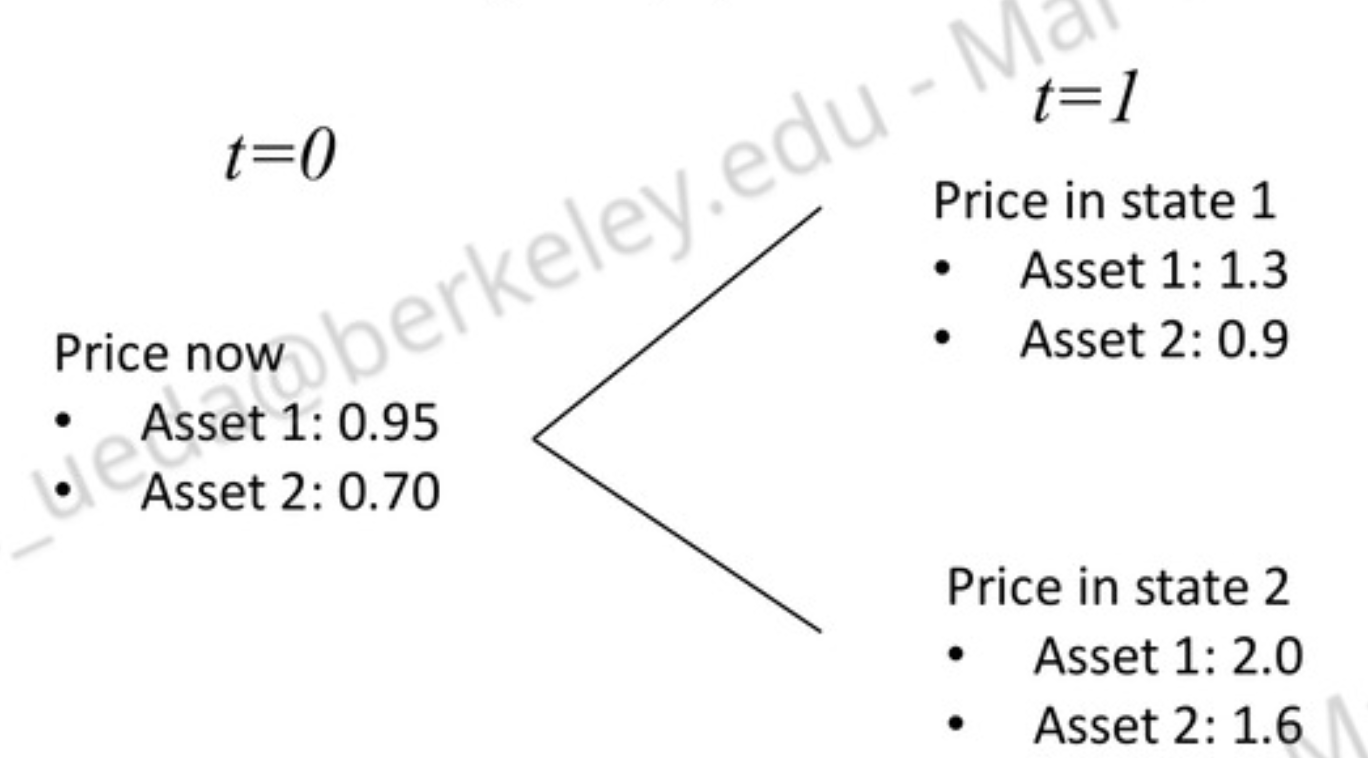
\includegraphics[width=4in]{imgs/example1.png}
    \caption{One Period, Two State Model}
\end{figure}

\begin{enumerate}
    \item Is the market complete? \\
    Approach: True if $\text{Rank}(\boldsymbol{D})=M$ (since this is a square matrix, this is 
    also true if $\boldsymbol{D}$ is invertible).
    \[
    \boldsymbol{D} = \begin{bmatrix}
        1.3 & 2.0 \\ 
        0.9 & 1.6
    \end{bmatrix}
    \] 
    $\text{Rank}(\boldsymbol{D})=2=M \rightarrow$ the market is complete.
    
    An equivalent check is that $\text{det}(\boldsymbol{D}) = ad - bc = (1.3 \times 1.6) - (2.0
    \times 0.9) = 0.28 \ne 0 \rightarrow \boldsymbol{D}$ is invertible and therefore the
    market is complete.
    \item What are the state prices? \\
    Approach: Find the state price vector.
    \[
    \boldsymbol{s}^0 = 
    \begin{bmatrix}
        0.95 \\ 
        0.70
    \end{bmatrix}, \;    
    \boldsymbol{D} = \begin{bmatrix}
        1.3 & 2.0 \\ 
        0.9 & 1.6
    \end{bmatrix}
    \]
    \[
    \boldsymbol{D}^{-1} =    
    {\begin{bmatrix}
        1.3 & 2.0 \\ 
        0.9 & 1.6
    \end{bmatrix}}^{-1} = \frac{1}{(1.3 \times 1.6) - (2.0 \times 0.9)} 
    \begin{bmatrix}
        1.6 & -2.0 \\
        -0.9 & 1.3
    \end{bmatrix} = \frac{1}{0.28}
    \begin{bmatrix}
        1.6 & -2.0 \\
        -0.9 & 1.3
    \end{bmatrix} = 
    \begin{bmatrix}
        5.714 & -7.143 \\
        -3.214 & 4.643
    \end{bmatrix} 
    \]
    
    \[ \boldsymbol{s}^0 = \boldsymbol{D}\psi \]
    Since $\boldsymbol{D}$ is square and invertible, we can find the SPV by solving for 
    \[
    \psi = \boldsymbol{D}^{-1}\boldsymbol{s}^0
    = \begin{bmatrix}
        5.714 & -7.143 \\
        -3.214 & 4.643
    \end{bmatrix} 
    \begin{bmatrix}
        0.95 \\ 
        0.70
    \end{bmatrix} =
    \begin{bmatrix}
        0.4282 \\
        0.1968
    \end{bmatrix}
    \]
    where $\psi_1=0.4282$ is the price for state 1 and $\psi_2=0.1968$ is the price for state 2.
    \item What is the price of an asset that pays $\$1$ in each state of the world? \\
    Approach: Since we have $\psi$ and the market is complete, we can price any payoff 
    structure. We want to price the payoff where we are paid $\$1$ in each state. \\
    \[
    \boldsymbol{V}^1 = \begin{bmatrix}
        1 & 1 
    \end{bmatrix}
    \]
    \[
    \psi_1 \times 1 + \psi_2 \times 1 = 0.4282 + 0.1968 = 0.625
    \]
    If we wanted, we could easily calculate $R^f$ as $\frac{1}{0.625} = 1.6$ since we are
    paying $0.625$ at $t=0$ to get $\$1$ at $t=1$.
\end{enumerate}

\subsection{Example}
Given the following one period, two state model, answer the questions below. 
\begin{figure}[H] 
    \centering 
    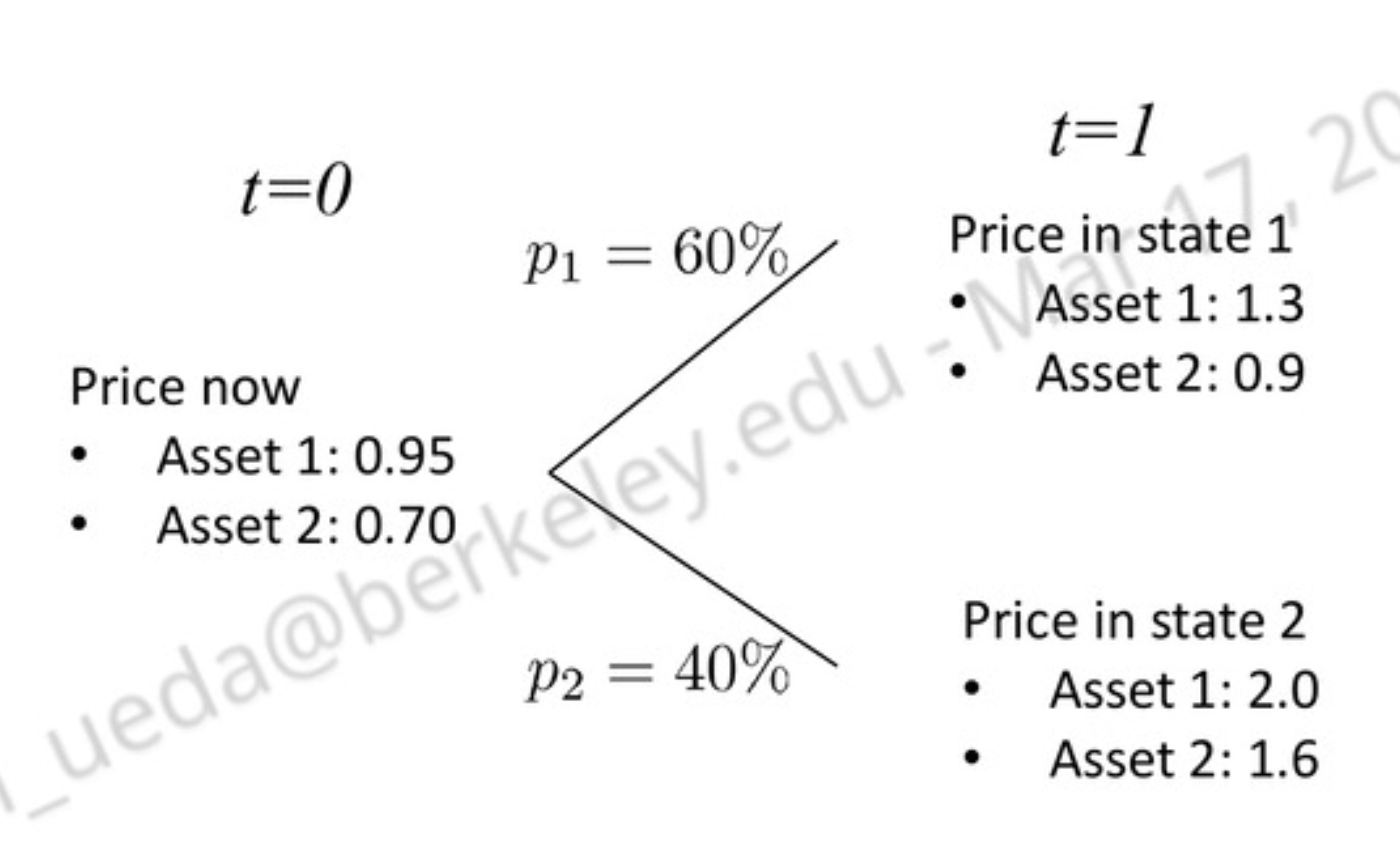
\includegraphics[width=4in]{imgs/example2.png}
    \caption{One Period, Two State Model}
\end{figure}

From example 1, we are also given 
\[
\psi = \begin{bmatrix}
    0.4282 \\ 
    0.1968
\end{bmatrix}    
\]
\[
    R^f = \frac{1}{\hat{\psi}} = \frac{1}{0.625} = 1.6
\]

\begin{enumerate}
    \item Find the equivalent martingale measure. \\
    Approach: The martingale measure is $\mathbb{Q}$, where each $q_i = \frac{\psi_i}
    {\hat{\psi}}$, and $\hat{\psi} = \sum_{i=1}^{M} \psi_i$.

    \[
    \hat{\psi} = \psi_1 + \psi_2 = 0.4282 + 0.1968 = 0.625 \\
    \]
    \[
    \begin{bmatrix}
        q_1 \\
        q_2
    \end{bmatrix} = 
    \begin{bmatrix}
        \frac{\psi_1}{\hat{\psi}} \\
        \frac{\psi_2}{\hat{\psi}}
    \end{bmatrix} = 
    \begin{bmatrix}
        0.4282/0.625 \\
        0.1968/0.625
    \end{bmatrix} = 
    \begin{bmatrix}
        0.685 \\
        0.315
    \end{bmatrix}
    \]
    \item Find the likelihood ratio. \\
    Approach: The likelihood ratio for each state $A$ is $L(A) = \frac{\mathbb{Q}(A)}
    {\mathbb{P}(A)}$.
    \[L(\omega_1) = \frac{q_1}{p_1} = \frac{0.685}{0.60} = 1.142\]
    \[L(\omega_2) = \frac{q_2}{p_2} = \frac{0.315}{0.40} = 0.7875\]

    \item Find the stochastic discount factor. \\
    Approach: The stochastic discount factor may be defined as $M_1 = \frac{1}{R}L$. 

    \[M_1(\omega_1) = \frac{1}{R} L(\omega_1) = \frac{1}{1.6} 1.142 = 0.714\]
    \[M_1(\omega_2) = \frac{1}{R} L(\omega_2) = \frac{1}{1.6} 0.7875 = 0.492\]
\end{enumerate}

\subsection{Example}

Answer the questions for the following economy

\[
\boldsymbol{s}^0 = 
\begin{bmatrix}
    1 \\ 
    1    
\end{bmatrix}, \; \boldsymbol{D} = 
\begin{bmatrix}
    5 & 5 & 5 & 5 & 5 \\
    3 & 3 & 3 & 3 & 7 
\end{bmatrix}
\]

\begin{enumerate}
    \item Is the market complete? \\ 
    Approach: If $\text{Rank}(\boldsymbol{D}) = M$, market is complete. Also, if there are
    fewer assets than there are states, that is $N < M$, the market cannot possibly be complete
    since the rank can be at most $\text{min}\{N, M\}$. \\

    Since $N<M$, we automatically know the market is not complete. 
    \item Is there an arbitrage opportunity? \\
    Approach: We could either think of this as trying to find  strictly positive SPV and then 
    use the FTAP or we could try to create an arbitrage and see if we could do it (this is 
    what we will do in this example since there aren't many states and assets to check and it 
    is an illustrative example this way). \\

    Recall: An arbitrage opportunity exists if there is some portfolio $\boldsymbol{h}$ such 
    that $\boldsymbol{h}^T \boldsymbol{\bar{D}} > 0 $. 

    The higher $M$ is, the more states we have to check, notice that really, in this example, 
    there are only 3 states we need to check (since states 1-4 have exactly the same payoffs), 
    which make up the new reduced matrix 

    \[
    \boldsymbol{\bar{D}} = 
    \begin{bmatrix}
        -1 & 5 & 5 \\
        -1 & 3 & 7 
    \end{bmatrix}    
    \]

    We now want to try to find some $\boldsymbol{h} = \begin{bmatrix} h_1 \\ h_2 \end{bmatrix}$
    such that $\boldsymbol{h}^T \boldsymbol{\bar{D}} > 0$.
    
    This provides us with 3 constraints:
    \[
    \boldsymbol{h}^T \boldsymbol{\bar{D}}  =
    \begin{bmatrix}
        h_1 & h_2 
    \end{bmatrix}
    \begin{bmatrix}
        -1 & 5 & 5 \\
        -1 & 3 & 7 
    \end{bmatrix} = 
    \begin{bmatrix}
        -h_1 - h_2 & 5h_1 + 3h_2 & 5h_1 + 7h_2
    \end{bmatrix} > 0
    \]

    Splitting these constraints apart, these say 
    \[-h_1 - h_2 > 0 \rightarrow h_1 + h_2 \le 0\]
    \[5h_1 + 3h_2 \ge 0\]
    \[5h_1 + 7h_2 \ge 0\]

    For $\boldsymbol{h}^T \boldsymbol{\bar{D}} > 0$ hold, we also need one of the above to be a
    strict inequality.

    \begin{figure}[H] 
        \centering 
        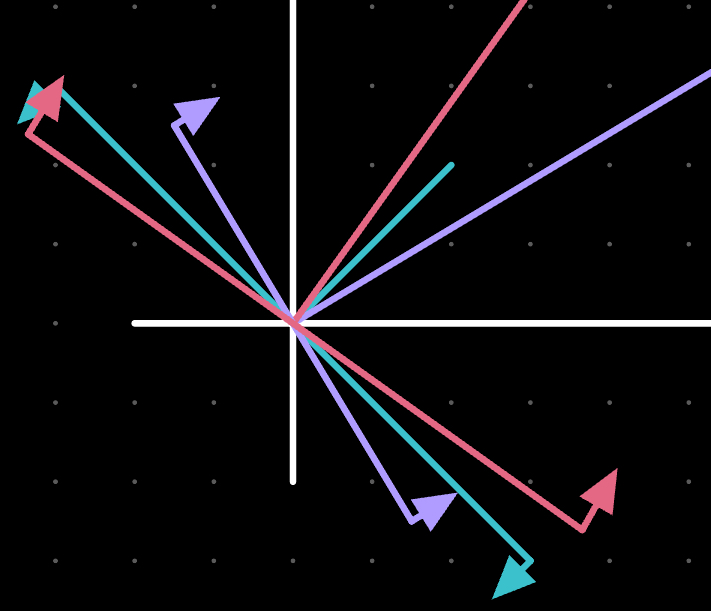
\includegraphics[width=4in]{imgs/example3.jpeg}
        \caption{Turquoise corresponds to vector [1, 1], purple corresponds with vector [5,3], 
        and red corresponds with vector [5,7]. The arrows denote the direction where the 
        constraint is met for each vector.}
    \end{figure}

    The image shows there are indeed no portfolios that satisfy all 3 constraints (other than 
    the origin, which is irrevelant since that is the case where we don't have any portfolio) 
    and therefore there is no way to satisfy $\boldsymbol{h}^T \boldsymbol{\bar{D}} > 0$. This
    allows us to conclude there is no arbitrage.
    \item Is there a strictly positive state price vector? \\
    Approach: By FTAP, we know the market if arbitrage free iff there exists a strictly
    positive SPV. Since we have shown the market is arbitrage free, we know there is a strictly 
    positive SPV. 

    Yes
    
\end{enumerate}

\subsection{Example}

Answer the questions for the following economy

\[
\boldsymbol{s}^0 = 
\begin{bmatrix}
    1 \\ 
    2 \\ 
    3 \\ 
    4 \\
    5  
\end{bmatrix}, \; \boldsymbol{D} = 
\begin{bmatrix}
    5 & 5 \\ 
    6 & 9 \\ 
    8 & 11 \\ 
    9 & 10 \\ 
    11 & 6 
\end{bmatrix}
\]

\begin{enumerate}
    \item Is the market complete? \\
    Approach: If $\text{Rank}(\boldsymbol{D}) = M$, market is complete. \\
    $\text{Rank}(\boldsymbol{D}) = 2 = M$ therefore, the market is complete.
    \item Is there an arbitrage opportunity? \\
    Approach: To show there exists an arbitrage, we just need to show one example, that is, one
    portfolio such that $\boldsymbol{h}^T \boldsymbol{\bar{D}} > 0$ \\ 

    Let 
    \[
    \boldsymbol{h} = \begin{bmatrix}
        2 \\
        -1 \\ 
        0 \\ 
        0 \\ 
        0
    \end{bmatrix}
    \]
    \[
    \boldsymbol{h}^T \boldsymbol{\bar{D}} = 
    \begin{bmatrix}
        2 & -1 & 0 & 0 & 0 
    \end{bmatrix}
    \begin{bmatrix}
        -1 & 5 & 5 \\ 
        -2 & 6 & 9 \\ 
        -3 & 8 & 11 \\ 
        -4 & 9 & 10 \\ 
        -5 & 11 & 6 
    \end{bmatrix} =
    \begin{bmatrix}
        -2+2 & 10-6 & 10-9
    \end{bmatrix} =
    \begin{bmatrix}
        0 & 4 & 1
    \end{bmatrix} > 0
    \]
    Therefore, we have shown that there is arbitrage in this economy since we have found a 
    portfolio such that $\boldsymbol{h}^T \boldsymbol{\bar{D}} > 0$.
    \item Is there a strictly positive state price vector? \\
    Approach: By FTAP, we know the market if arbitrage free iff there exists a strictly
    positive SPV. Since we have shown the market is not arbitrage free, we know there is not a 
    strictly positive SPV. 
\end{enumerate}

\subsection{Example}

Given the following 1 period, 2 state binomial tree market (denoted by the image below).

\begin{figure}[H] 
    \centering 
    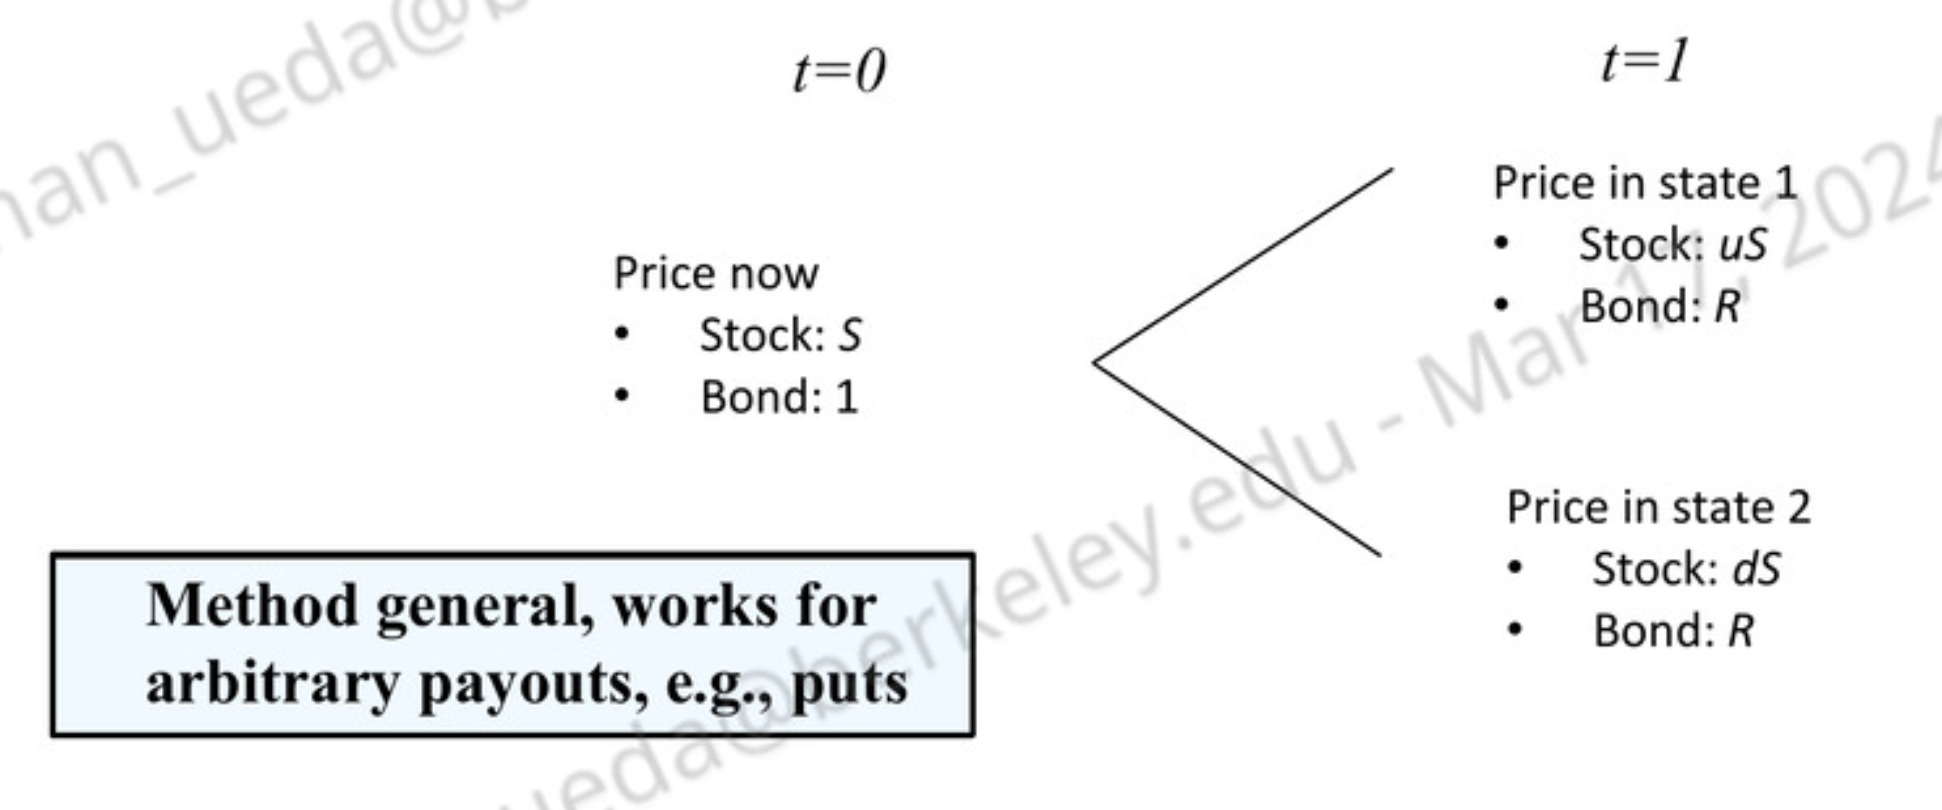
\includegraphics[width=4in]{imgs/one_period_two_state_bin_tree_model.png}
    \caption{Price dynamics}
\end{figure}

This can be setup as 
    \[
    \boldsymbol{s}_0 = \begin{bmatrix}
        1 \\ 
        1
    \end{bmatrix}
    \]
    \[ 
    \boldsymbol{D} = \begin{bmatrix}
        u & d \\
        R & R \\
    \end{bmatrix}
    \]

For this $2 \times 2$ market, answer the following questions.
\begin{enumerate}
        \item What are the conditions for noarbitrage?
        \begin{itemize}
            \item No arbitrage if $d < R < u$: If $R$ is greater than $u$ and $d$, then there 
            would be no reason to take on the risk of the stock since more could be earned risk 
            free with $R$. If $R$ is less than $u$ and $d$, then the stock is superior. 
            \item Another possibility for a market with no arbitrage would be if $d = R = u$. 
            The market would not be complete, but there would be no arbitrage.
        \end{itemize}
        \item What are the conditions for a complete market? \\
        Approach: If $\text{Rank}(\boldsymbol{D}) = M$, market is complete. \\

        $u \ne d$. If $u=d$, $\text{Rank}(\boldsymbol{D}) = 1 < M = 2$.
        \item What are the state prices? \\
        Approach: Find the state price vector. Since this is a $2 \times 2$ market, we can just 
        invert $\boldsymbol{s}^0 = \boldsymbol{D}\psi$ and solve for $\psi = 
        \boldsymbol{D}^{-1} s^0$ to get the state prices. \\
        
        Recall
        \[
        {\begin{bmatrix}
            a & b \\
            c & d 
        \end{bmatrix}}^{-1} = 
        \frac{1}{ad - bc} 
        \begin{bmatrix}
            d & -b \\ 
            -c & a
        \end{bmatrix}
        \] \\
        Therefore
        \[
        \boldsymbol{D}^{-1} = \frac{1}{uR - Rd} 
        \begin{bmatrix}
            R & - d \\ 
            -R & u
        \end{bmatrix} = 
        \boldsymbol{D}^{-1} = \frac{1}{(u - d)R} 
        \begin{bmatrix}
            R & - d \\ 
            -R & u
        \end{bmatrix}
        \]

        \[
        \psi = \boldsymbol{D}^{-1} s^0 = \frac{1}{(u - d)R} 
        \begin{bmatrix}
            R & - d \\ 
            -R & u
        \end{bmatrix} 
        \begin{bmatrix}
            1 \\ 
            1
        \end{bmatrix} = \frac{1}{(u - d)R} 
        \begin{bmatrix}
            R - d \\ 
            u - R
        \end{bmatrix} = 
        \begin{bmatrix}
            \frac{R-d}{(u-d)R} \\
            \frac{u-R}{(u-d)R} \\
        \end{bmatrix}
        \]
    
        \item What are the risk neutral probabilities? \\
        Approach: The risk neutral measure is $\mathbb{Q}$, where each $q_i = \frac{\psi_i}
        {\hat{\psi}}$, and $\hat{\psi} = \sum_{i=1}^{M} \psi_i$. \\
    
        Calculate 
        \[
        \hat{\psi} = \psi_1 + \psi_2 
        = \frac{R-d}{(u-d)R} + \frac{u-R}{(u-d)R} 
        = \frac{R-d+u-R}{(u-d)R} 
        = \frac{u-d}{(u-d)R} 
        = \frac{1}{R} 
        \]
        \[q_u = \frac{\psi_1}{\hat{\psi}} = \frac{R-d}{u-d}\]
        \[q_d = \frac{\psi_2}{\hat{\psi}} = \frac{u-R}{u-d}\]
        Therefore 
        \[
        \begin{bmatrix}
            q_u \\
            q_d 
        \end{bmatrix} =
        \begin{bmatrix}
            \frac{R-d}{u-d} \\
            \frac{u-R}{u-d}
        \end{bmatrix}    
        \]
        The $q_u$ is the $q$ for an up move, is typically what we call the risk neutral 
        probability.
        
        \item What is the price the call option?
        \[
        C_0 = C_u \psi_1 + C_d \psi_2
        = \frac{1}{R} E_{\mathbb{Q}}[\tilde{C}_1] 
        = \frac{1}{R} (C_u q_u + C_d q_d)
        \]
        
        
    
    \item Payoff for call will be either 
    \[C_u = \text{max}(uS - K, 0)\]
    or 
    \[C_d = \text{max}(dS - K, 0)\]
\end{enumerate}

\subsection{Example}

Given the following 1 period, 2 state binomial tree market (denoted by the image below).

\begin{figure}[H] 
    \centering 
    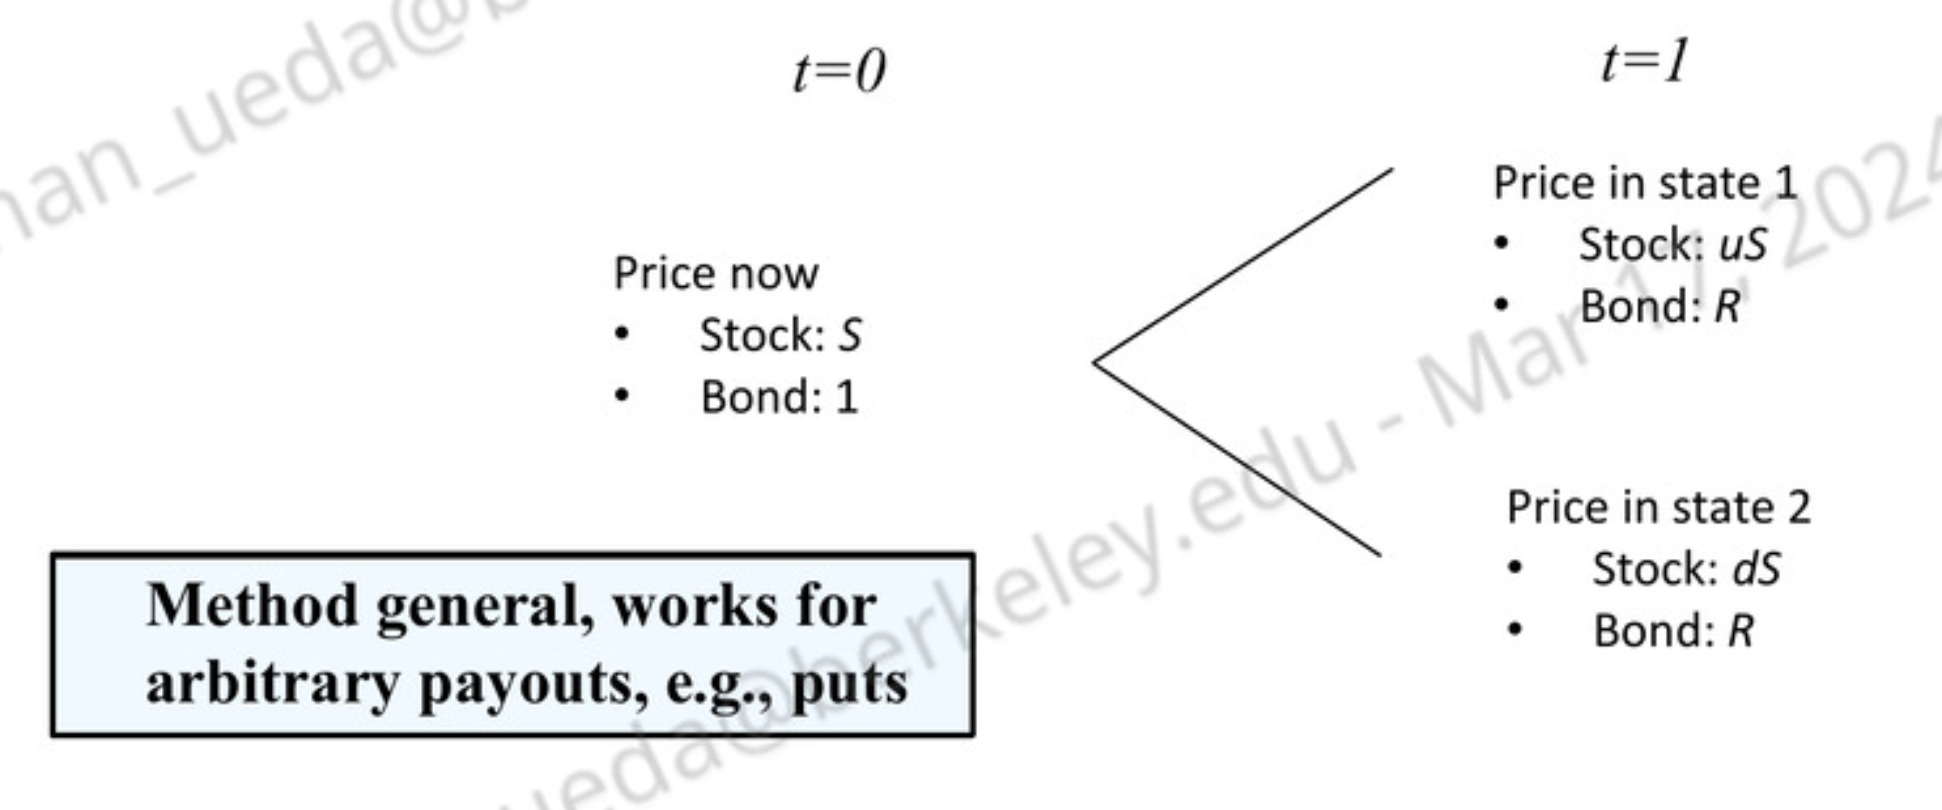
\includegraphics[width=4in]{imgs/one_period_two_state_bin_tree_model.png}
    \caption{Price dynamics}
\end{figure}

Note that an equivalent interprestion, since payoff is in $\boldsymbol{\mathcal{R}}$, should be 
possible to form a \textit{replciating portfolio}, $\boldsymbol{h}= 
\begin{bmatrix}
    \Delta \\
    B
\end{bmatrix}$, where $\Delta$ is the number of shares bought at $B$ is how much is put into 
the bond.

Conditions we want for the payoff are
\[\Delta u S + B R = C_u\] 
\[\Delta d S + B R = C_d\]

The price today of the portfolio must be equal to the price of the call for there to be no 
arbitrage, that is
\[C = \Delta S + B \]

Solve for $\Delta$

\begin{align*}
    (\Delta u S + B R) - (\Delta d S + B R) &= C_u - C_d \\
    \Delta S (u-d) &= C_u - C_d \\ 
    \Delta &= \frac{C_u - C_d}{S (u-d)}
\end{align*}

Plug $\Delta$ into the first equation 

\begin{align*}
    \Delta u S + B R &= C_u \\
    \frac{C_u - C_d}{S (u-d)} u S + B R &= C_u \\
    \frac{C_u - C_d}{(u-d)} u + B R &= C_u \\
    C_u u- C_d u + B R(u-d) &= C_u(u-d) \\
    C_u u- C_d u + B R(u-d) &= C_u u - C_u d \\
    B R(u-d) &= C_u u - C_u d - C_u u + C_d u \\
    B R(u-d) &= C_d u- C_u d \\
    B &= \frac{C_d u- C_u d}{R(u-d)}
\end{align*}

Plug in $\Delta$ and $B$ into the equation for $C$

\begin{align*}
    C &= \Delta S + B \\
    C &= \frac{C_u - C_d}{S (u-d)} S + \frac{C_u u- C_u d}{R(u-d)} \\
    C &= \frac{C_u - C_d}{S (u-d)} S \frac{R}{R} + \frac{C_u u- C_u d}{R(u-d)} \\
    C &= \frac{RC_u - RC_d}{R(u-d)} + \frac{C_u u- C_u d}{R(u-d)} \\
    C &= \frac{RC_u - RC_d + C_u u - C_u d}{R(u-d)} \\
    C &= C_u \frac{R-d}{R(u-d)} + C_d\frac{u-R}{R(u-d)} \\
\end{align*}

\subsection{Example}
Given the following 2 period binomial model 

\begin{figure}[H] 
    \centering 
    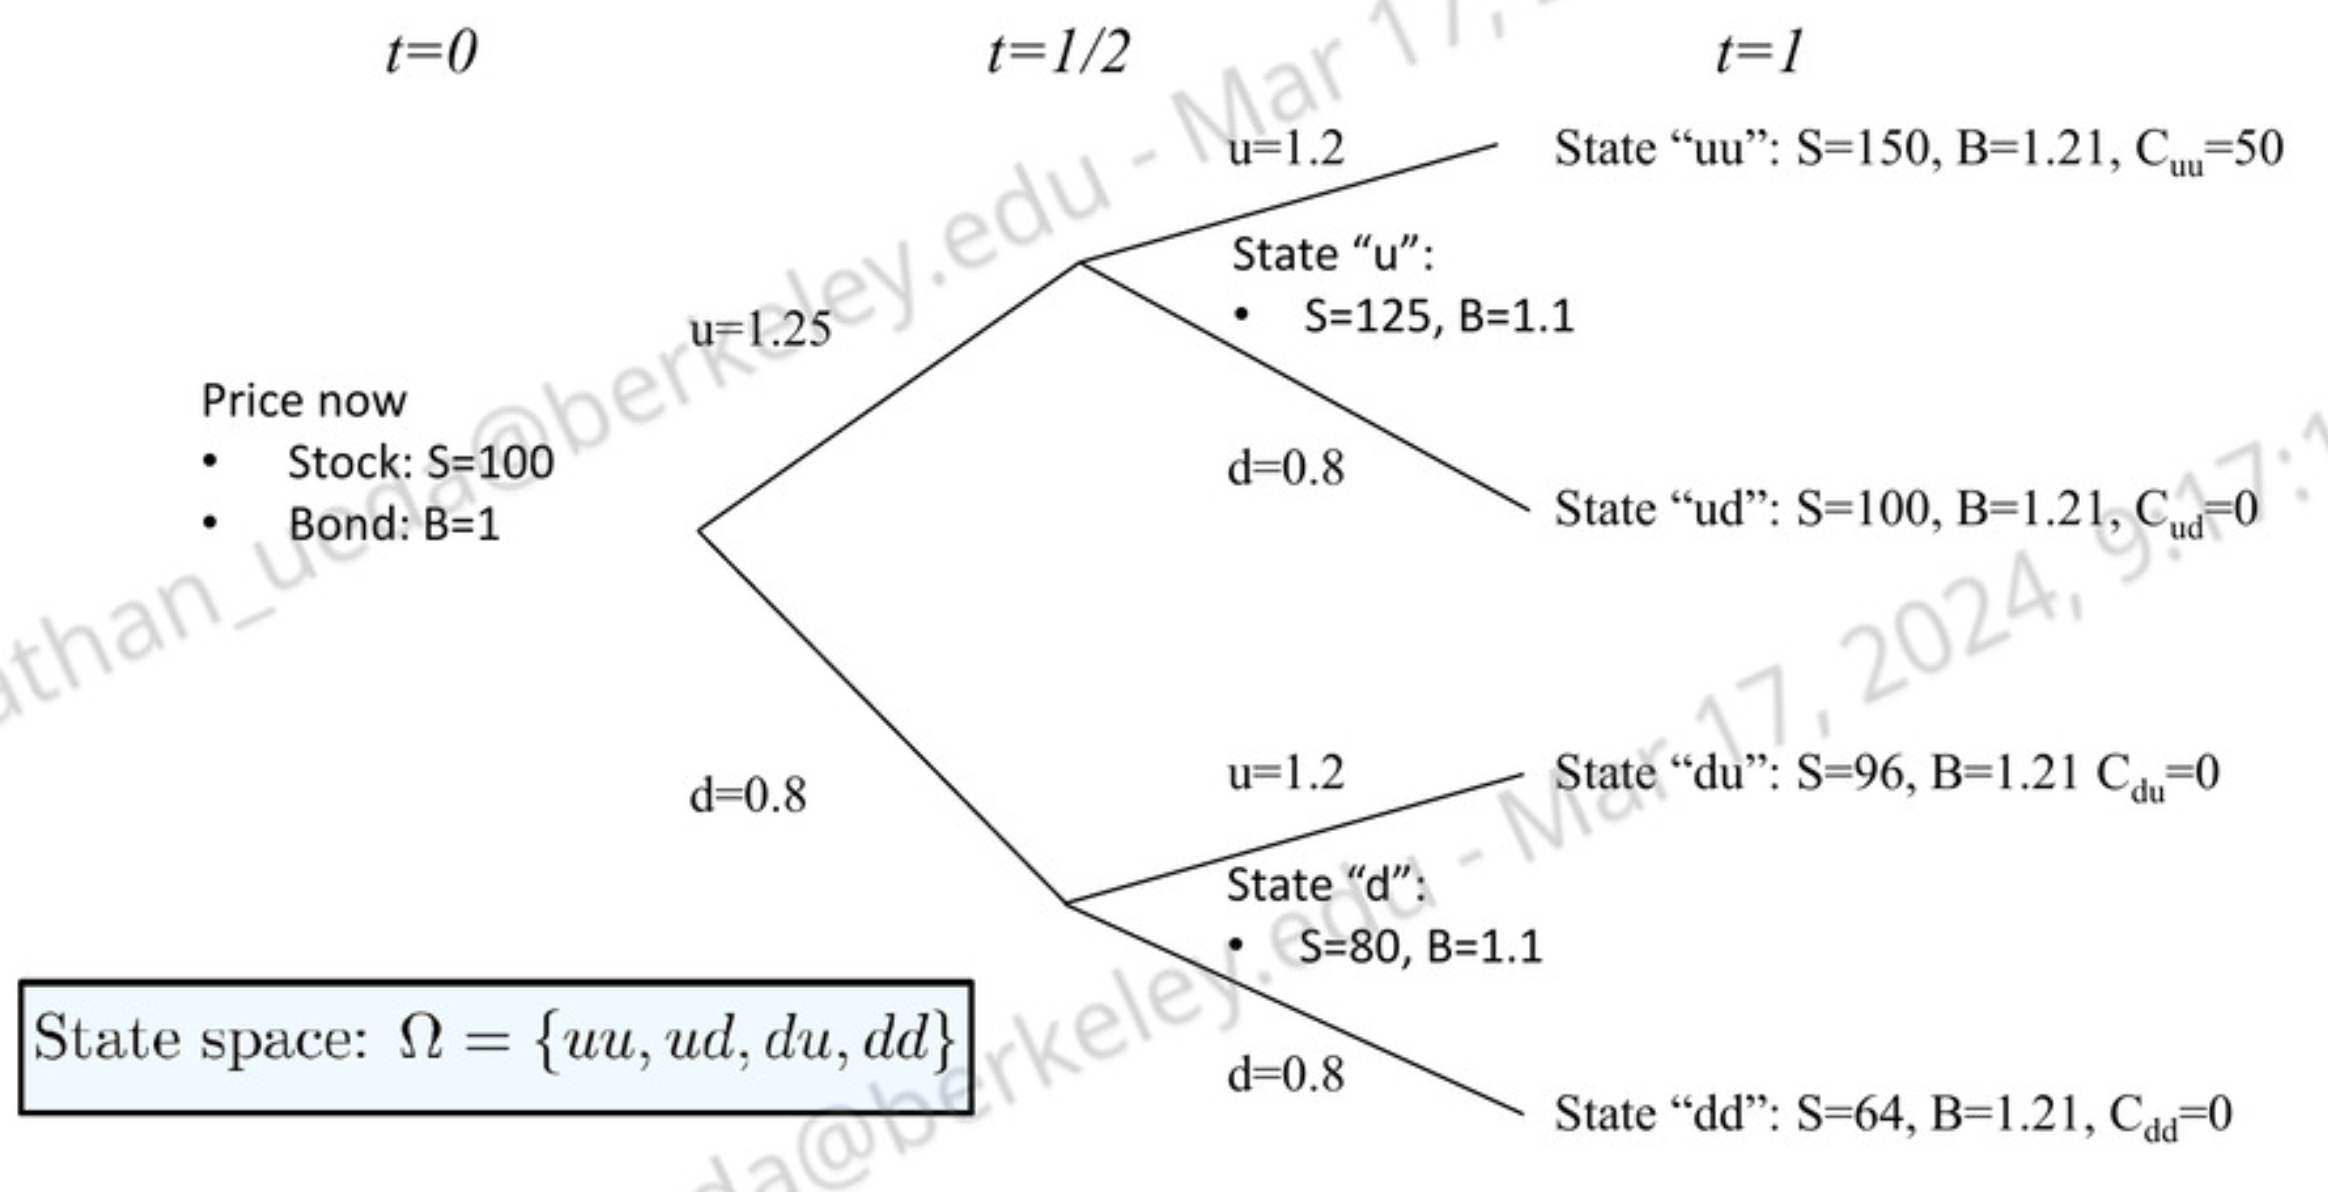
\includegraphics[width=5in]{imgs/two_period_two_state_bin_tree_model.png}
    \caption{Two period binomial model}
\end{figure}

Approach: To analyze this, the easiest method would be to split it into a series of single 
period models. For the structure of this tree, that would be 3 single period models. Solving 
for each of these will give us the unique value of the call option at time $t=0$. \\

We start by analyzing the dynamics from $t=1/2$ to $t=1$ after an up move. 

\begin{figure}[H] 
    \centering 
    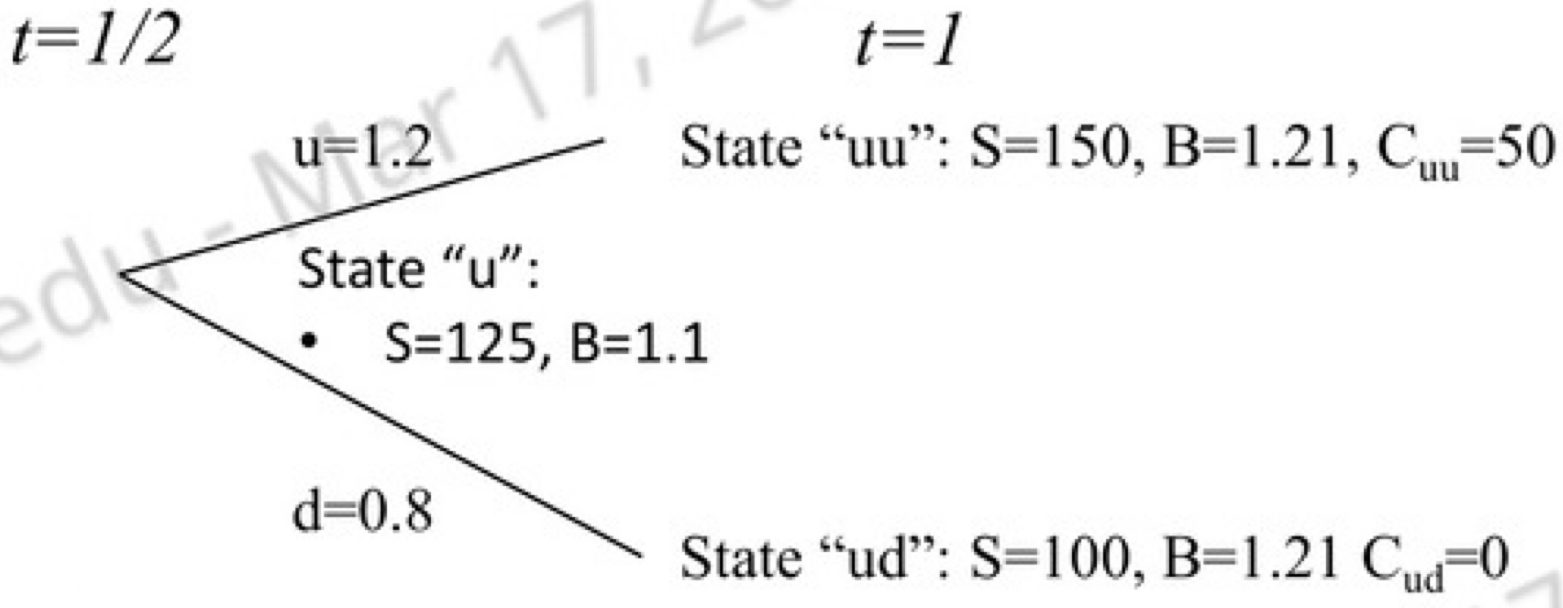
\includegraphics[width=4in]{imgs/two_period_two_state_bin_tree_model_up.jpeg}
    \caption{The one period model at time $t=1/2$ to $t=1$ after an up move}
\end{figure}
% Always denoting bond as 1 dollar
\[ 
    \boldsymbol{s}^0 = 
    \begin{bmatrix}
        125 \\ 
        1     
    \end{bmatrix}, \;
    \boldsymbol{D} = 
    \begin{bmatrix}
        150 & 100 \\
        1.1 & 1.1 
    \end{bmatrix}
\]

\begin{enumerate}
    \item Calculate the risk neutral probability:
    \[
      q_u = \frac{R-d}{u-d} = \frac{1.1-0.8}{1.2-0.8} = \frac{3}{4}   
    \]
    \item Calculate the price of the call option after the up move, $C_u$ at time $t=1/2$
    \[
      C_u = \frac{1}{R}(C_{uu} q_u + C_{ud} (1-q_u))
      = \frac{1}{1.1} (50 \times 0.75 + 0 \times 0.25)  
      = 34.1
    \]
    \item Calculating the replicating portfolio \\
    Approach: Since we just had an up move, we are now calculating this at time $t=1/2$. The 
    replicating portfolio here states how to replicate a portfolio that has payments at $t=1$ of 
    $C_{uu}=50$ after two up total up-moves and $C_{ud} = 0$ after an up-move followed by a 
    down-move.
    
    Recall the formulas to calculate the amount of shares and bonds.
    \[\Delta = \frac{C_u - C_d}{S (u-d)}\]
    \[B = \frac{C_d u- C_u d}{R(u-d)}\]
    Apply these to our scenario and solve
    \[
    \Delta_u = \frac{C_{uu} - C_{ud}}{S (u-d)} 
    = \frac{50 - 0}{125 \times (1.2-0.8)}
    = \frac{50}{50}
    = 1
    \]
    \[
    B_u = \frac{C_{ud}u - C_{uu} d}{R(u-d)}
    = \frac{(0 \times 1.2) - (50 \times 0.8)}{1.1(1.2-0.8)}
    = -\frac{40}{.44}
    = -90.91
    \]
\end{enumerate}

Second, we will analyzing the dynamics from $t=1/2$ to $t=1$ after a down move. 

\begin{figure}[H] 
    \centering 
    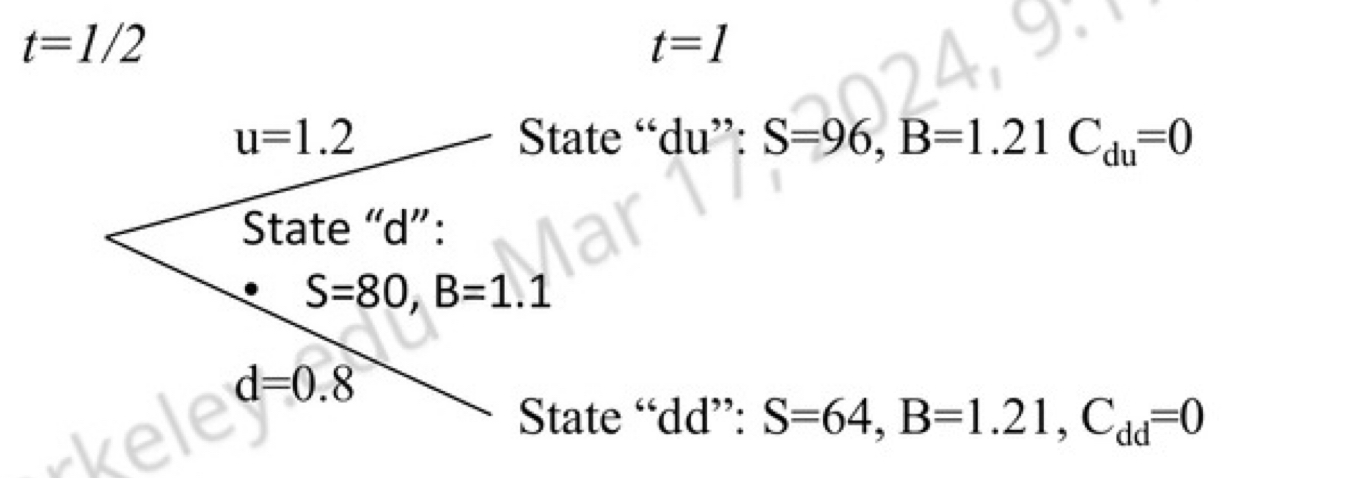
\includegraphics[width=4in]{imgs/two_period_two_state_bin_tree_model_down.jpeg}
    \caption{The one period model at time $t=1/2$ to $t=1$ after a down move}
\end{figure}

\[ 
    \boldsymbol{s}^0 = 
    \begin{bmatrix}
        80 \\ 
        1     
    \end{bmatrix}, \;
    \boldsymbol{D} = 
    \begin{bmatrix}
        96 & 64 \\
        1.1 & 1.1 
    \end{bmatrix}
\]

\begin{enumerate}
    \item Calculate the risk neutral probability:
    \[
      q_u = \frac{R-d}{u-d} = \frac{1.1-0.8}{1.2-0.8} = \frac{3}{4}   
    \]
    \item Calculate the price of the call option after the down move, $C_d$ at time $t=1/2$
    \[
      C_d = \frac{1}{R}(C_{du} q_u + C_{dd} (1-q_u))
      = \frac{1}{1.1} (0 \times 0.75 + 0 \times 0.25)  
      = 0
    \]
    \item Calculating the replicating portfolio \\
    Approach: Since we just had a down move, we are now calculating this at time $t=1/2$. The 
    replicating portfolio here states how to replicate a portfolio that has payments at $t=1$ of 
    $C_{du}=0$ after a down move followed up an up move and $C_{dd} = 0$ after two down moves.
    
    Recall the formulas to calculate the amount of shares and bonds.
    \[\Delta = \frac{C_u - C_d}{S (u-d)}\]
    \[B = \frac{C_d u- C_u d}{R(u-d)}\]
    Apply these to our scenario and solve
    \[
    \Delta_d = \frac{C_{du} - C_{dd}}{S (u-d)} 
    = \frac{0 - 0}{80 \times (1.2-0.8)}
    = 0
    \]
    \[
    B_d = \frac{C_{dd}u - C_{du} d}{R(u-d)}
    = \frac{(0 \times 1.2) - (0 \times 0.8)}{1.1(1.2-0.8)}
    = 0
    \]
\end{enumerate}

Lastly, we will analyzing the dynamics at time $t=0$.


\begin{figure}[H] 
    \centering 
    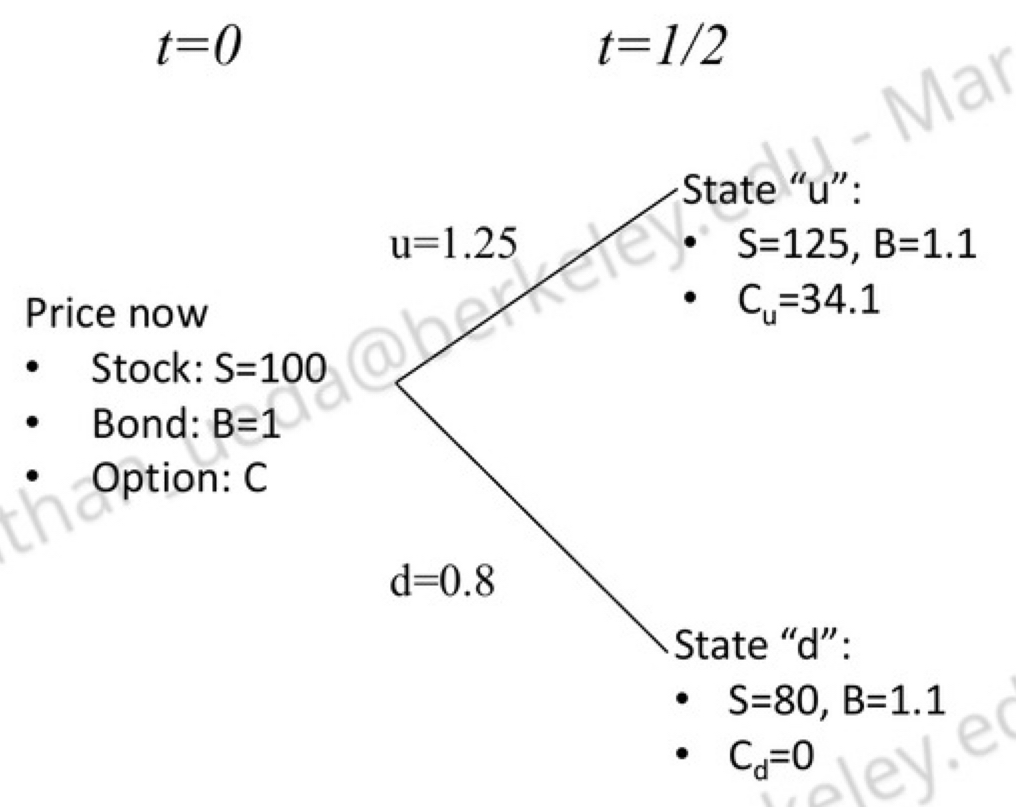
\includegraphics[width=4in]{imgs/two_period_two_state_bin_tree_model_initial.jpeg}
    \caption{The one period model at time $t=0$ to $t=1/2$}
\end{figure}

\[ 
    \boldsymbol{s}^0 = 
    \begin{bmatrix}
        100 \\ 
        1     
    \end{bmatrix}, \;
    \boldsymbol{D} = 
    \begin{bmatrix}
        125 & 80 \\
        1.1 & 1.1 
    \end{bmatrix}
\]

\begin{enumerate}
    \item Calculate the risk neutral probability:
    \[
      q_u = \frac{R-d}{u-d} = \frac{1.1-0.8}{1.25-0.8} = \frac{2}{3}   
    \]
    \item Calculate the price of the call option, $C$ at time $t=0$
    \[
      C = \frac{1}{R}(C_{u} q_u + C_{d} (1-q_u))
      = \frac{1}{1.1} (34.1 \times \frac{2}{3} + 0 \times \frac{1}{3})  
      = 20.67
    \]
    \item Calculating the replicating portfolio \\
    Approach: Since we haven't moved yet, we are calculating this at time $t=0$. The
    replicating portfolio here states how to replicate a portfolio that has payments at $t=1/2$ of 
    $C_{u}=34.1$ after an up-move and $C_{d} = 0$ after a down-move.
    
    Recall the formulas to calculate the amount of shares and bonds.
    \[\Delta = \frac{C_u - C_d}{S (u-d)}\]
    \[B = \frac{C_d u- C_u d}{R(u-d)}\]
    Apply these to our scenario and solve
    \[
    \Delta = \frac{C_{u} - C_{d}}{S (u-d)} 
    = \frac{34.1 - 0}{100 \times (1.25-0.8)}
    = \frac{34.1}{45}
    = 0.758
    \]
    \[
    B = \frac{C_{d}u - C_{u} d}{R(u-d)}
    = \frac{(0 \times 1.25) - (34.1 \times 0.8)}{1.1(1.25-0.8)}
    = -\frac{27.28}{.495}
    = -55.11
    \]
\end{enumerate}

In contrast to an incomplete market where, for the initial call we are only able to get bounds
for the option price, with a (dynamically) complete market we can nail down an exact figure. 
% A multiperiod model allows a trader to trade at even interval of $t$, essentially splitting the 
% multiperiod model into a series of single period models. 

% Dynamically complete mean that the reachable payoff space is the whole of R^m, if we are allowed To
% rebalance out portfolio over time 

\subsection{Example}

Given the following two period European put 

\begin{figure}[H] 
    \centering 
    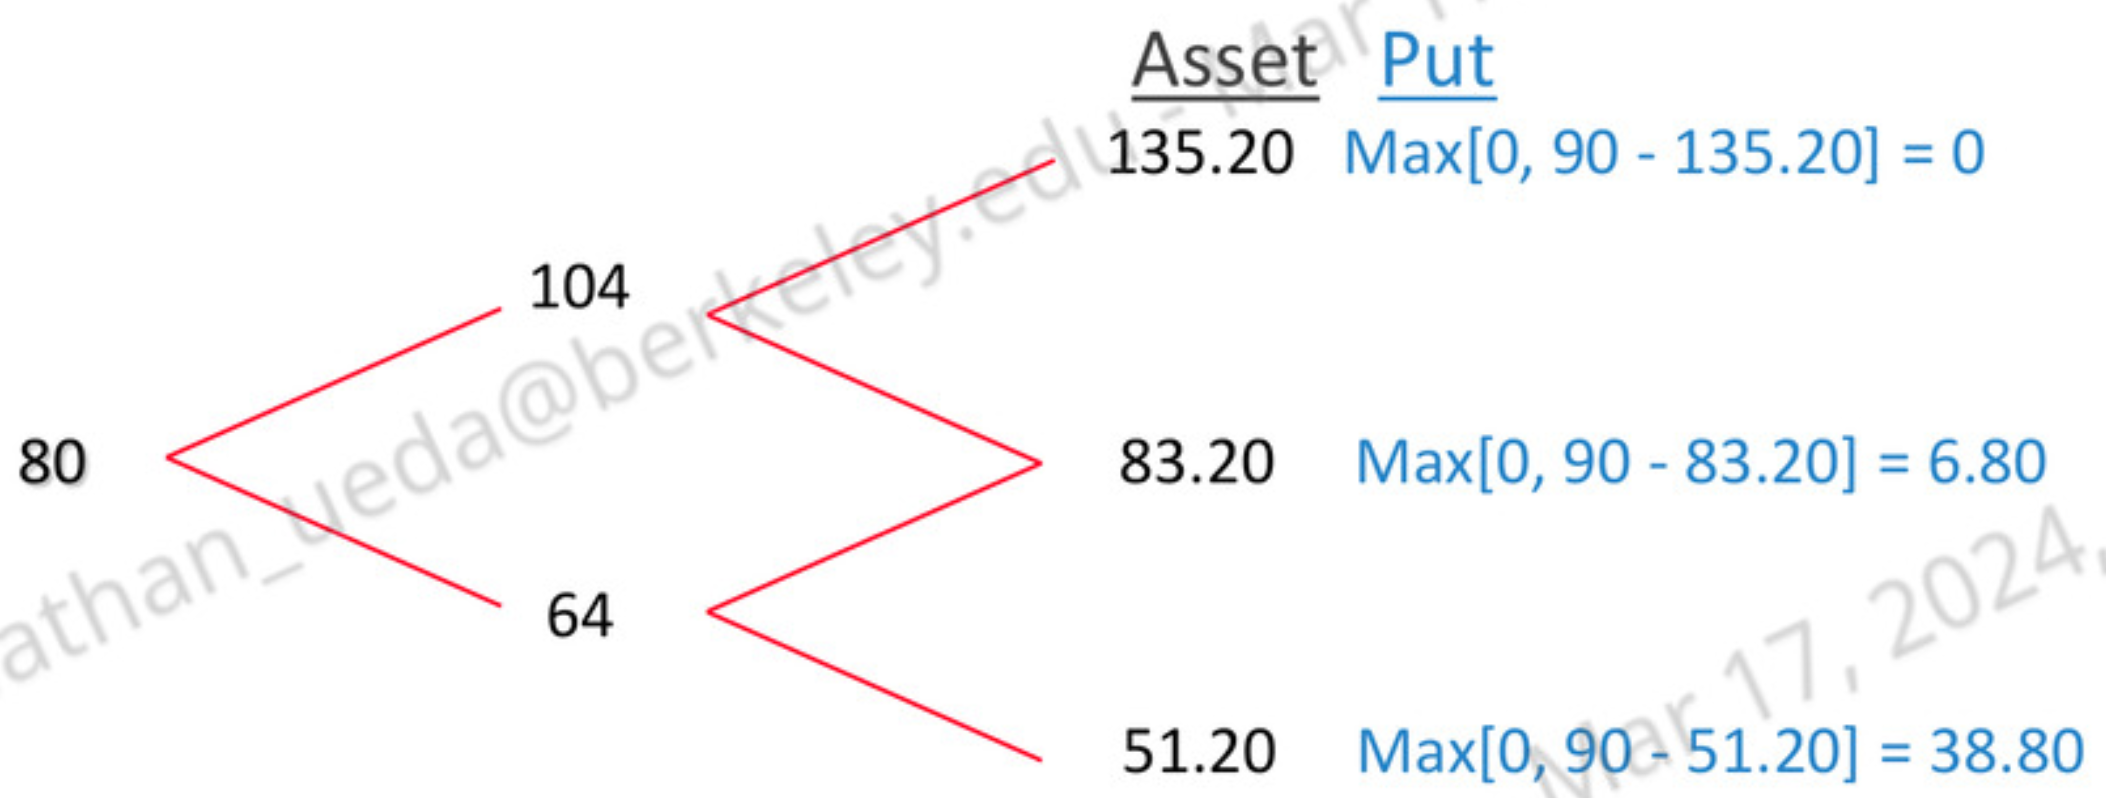
\includegraphics[width=4in]{imgs/two_period_euorpean_put.png}
    \caption{Two period European put labeled with the value of the stock, $S$} 
\end{figure}

\[S = 80, \; K = 90, \; R=1.1, \; u = 1.3, \; d = 0.8\]

Recall we are only able to exercise at the end. \\

Approach: Start and the end and work backwards through the tree. \\  

\[ Su = 80 \times 1.3 = 104 \]
\[ Sd = 80 \times 0.8 = 64 \]

\[\text{Put Payoff: Max}\{0, K - S\}\]

Therefore at the terminals, we have

\[P_{uu} = \text{Max}\{0, 90 - 135.20\} = 0\]
\[P_{ud} = P_{du} = \text{Max}\{0, 90 - 83.20\} = 6.80\]
\[P_{dd} = \text{Max}\{0, 90 - 51.20\} = 38.80\]

With this information, we may now price the puts at the period prior, $P_u, P_d, P$, using the
risk neutral formula $q_u = \frac{R-d}{u-d}$

\[
q_u = \frac{R-d}{u-d}
= \frac{1.1-0.8}{1.3-0.8}
= 0.6
\]

We can calculate the prices of $P_u, P_d$

\[
P_u = \frac{1}{R}(q_u P_{uu} + (1-q_u) P_{ud})
= \frac{1}{1.1}(0.6 \times 0  + 0.4 \times 6.8)
= 2.473
\]

\[
P_d = \frac{1}{R}(q_u P_{du} + (1-q_u) P_{dd})
= \frac{1}{1.1}(0.6 \times 6.80 + 0.4 \times 38.80)    
= 17.818
\]

Finally, we can use $P_u, P_d$ to price $P$.

\[
P = \frac{1}{R}(q_u P_u + (1-q_u) P_d)
= \frac{1}{1.1}(0.6 \times 2.473 + 0.4 \times 17.818)
= 7.828
\]

\begin{figure}[H] 
    \centering 
    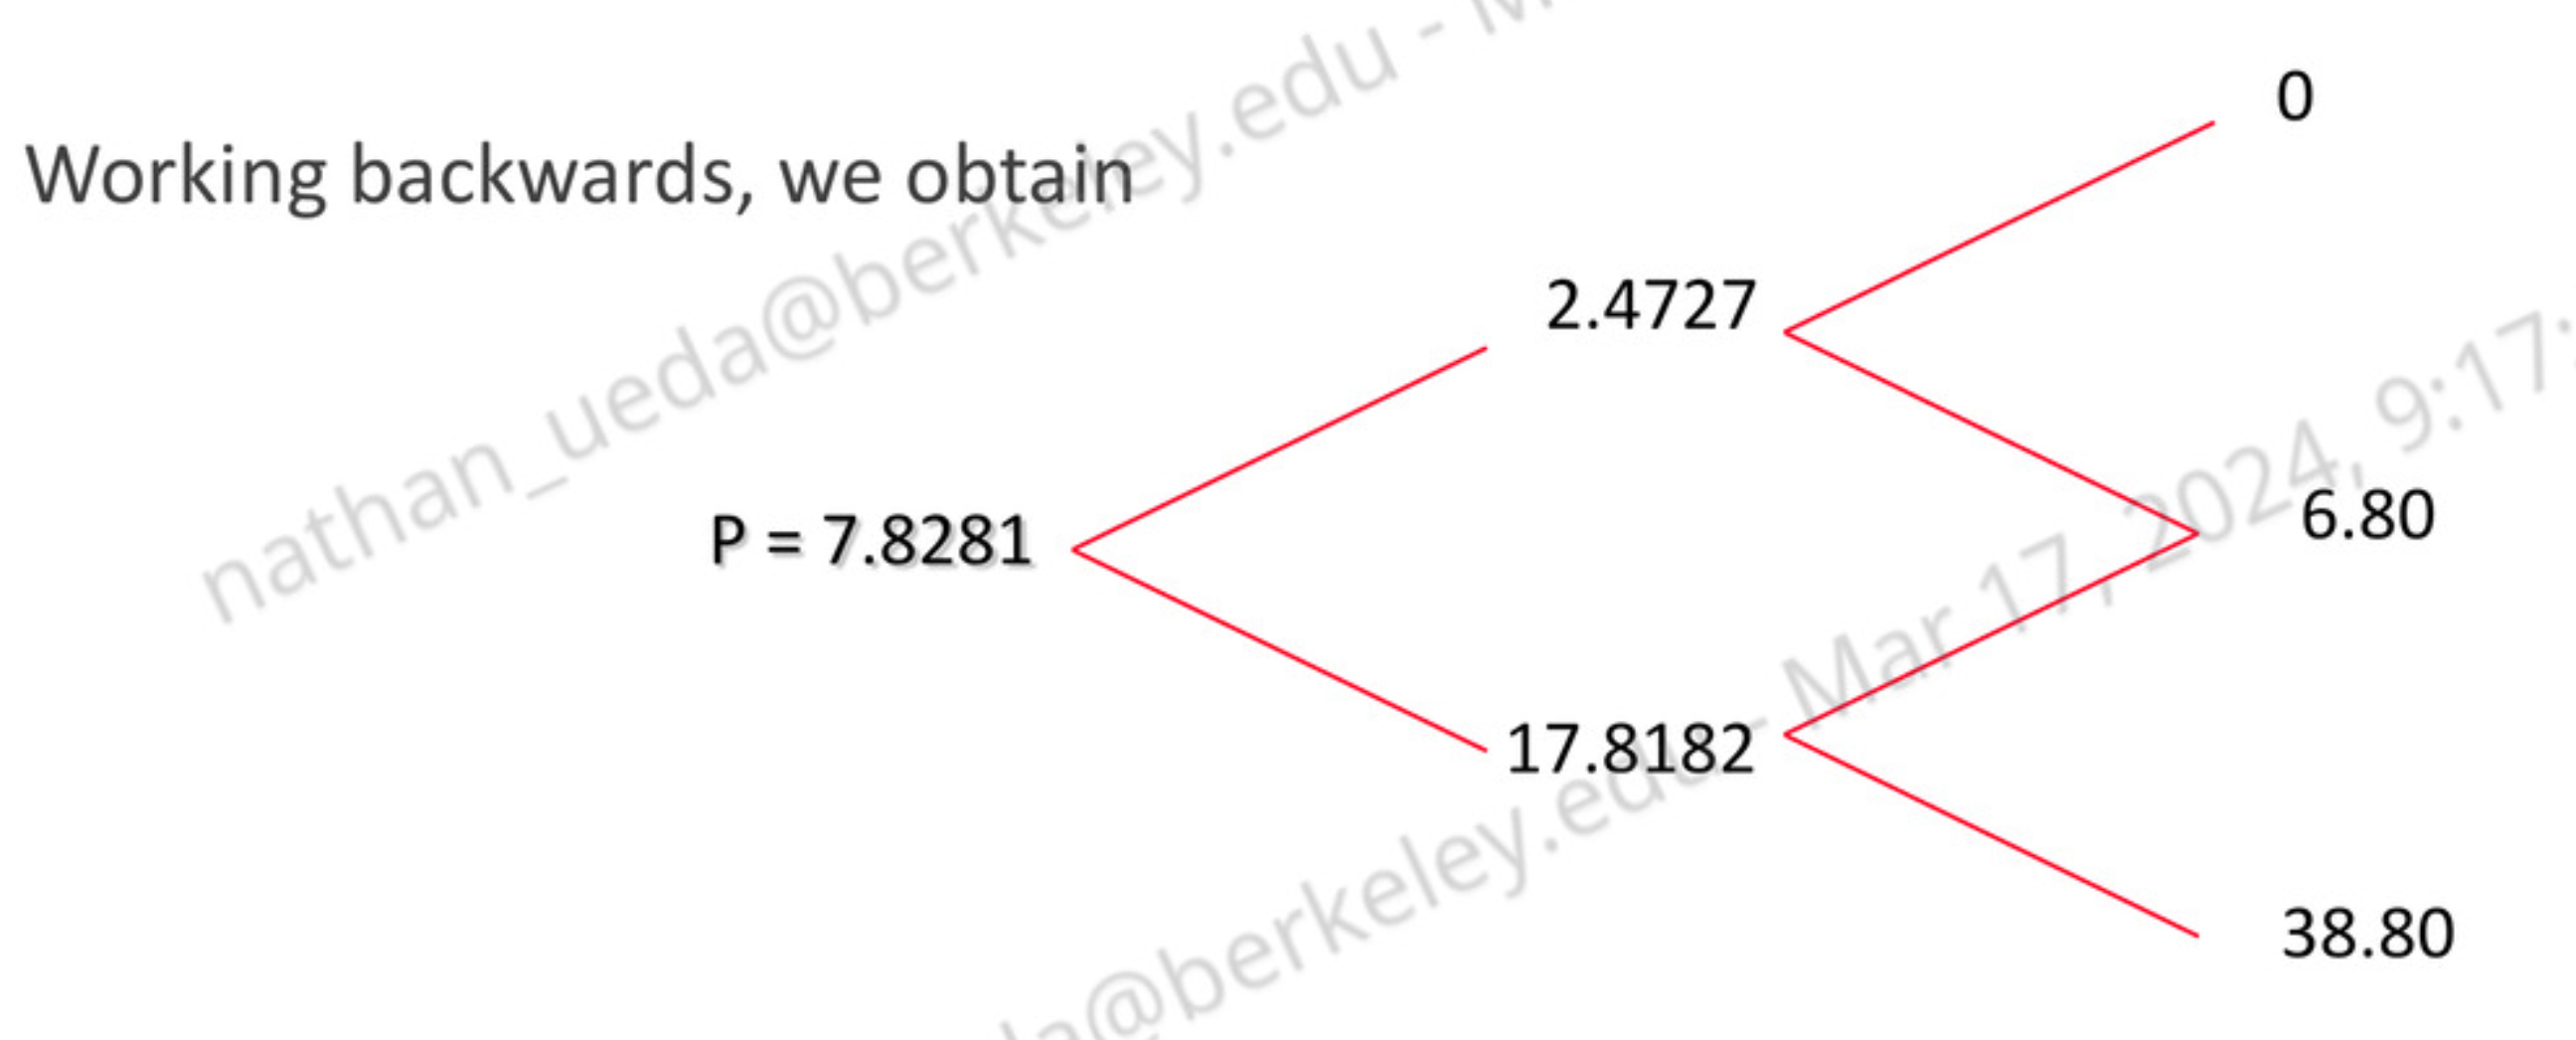
\includegraphics[width=4in]{imgs/two_period_euorpean_put_2.png}
    \caption{Two period European put labeled with the value of the puts} 
\end{figure}

With an American put, we have the opportunity to exercise early. 
So when moving backwards, we need to check if it is more valuable to 
exericse the option early. 

\begin{figure}[H] 
    \centering 
    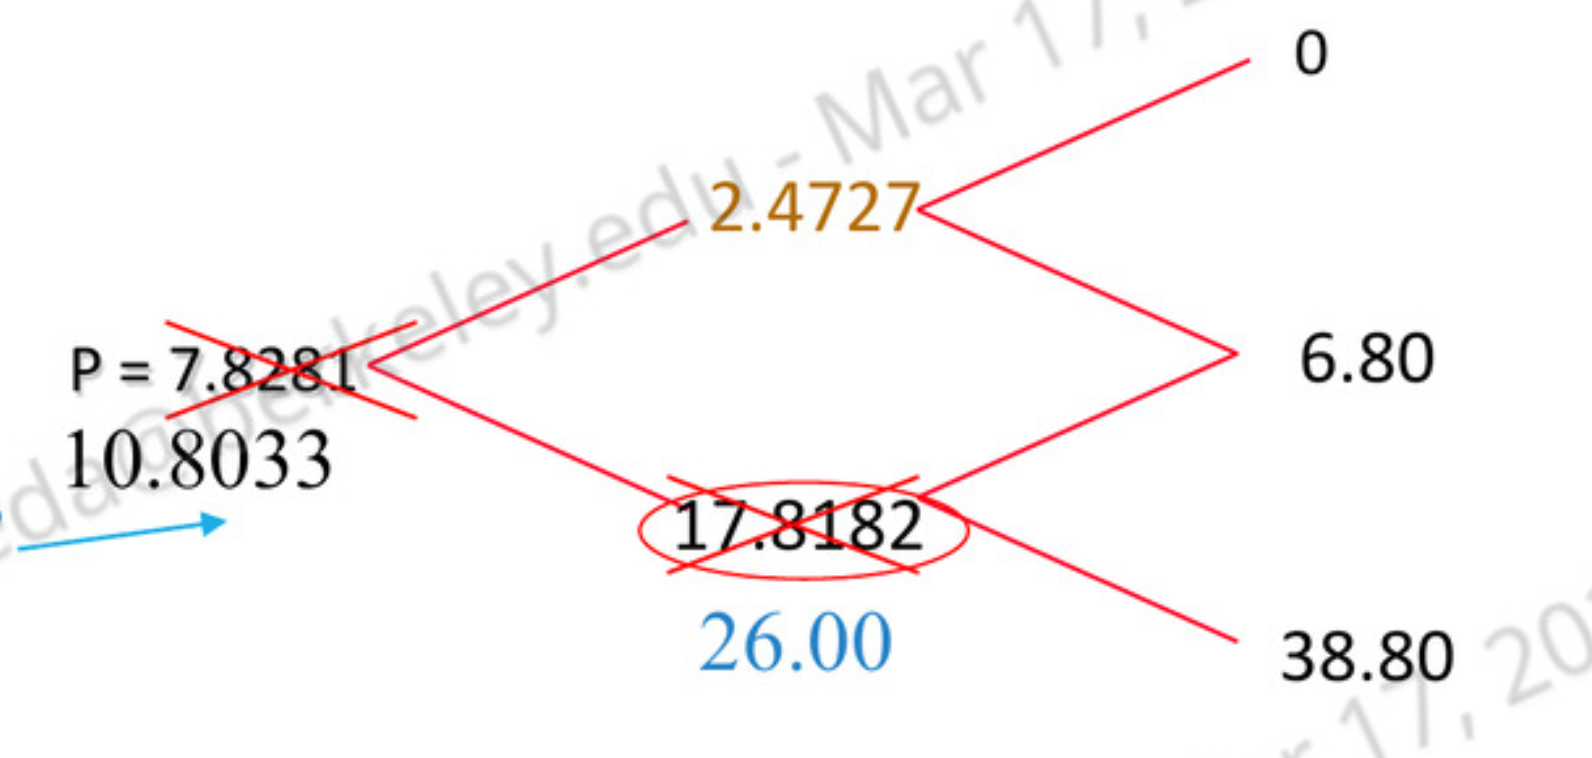
\includegraphics[width=4in]{imgs/two_period_american_put.png}
    \caption{Two period American put labeled with the value of the puts} 
\end{figure}

At time $t=1$

\[
P_u = \text{max}\{2.473, \text{max}\{K - S\}\}
= \text{max}\{2.473, \text{max}\{90 - 104\}\}
= 2.473
\]

\[
P_d = \text{max}\{17.818, \text{max}\{K - S\}\}
= \text{max}\{17.818, \text{max}\{90 - 64\}\}
= 26
\]

Therefore, the new value of $P$, taking into consideration the updated value of $P_u$ is
\[
P = \frac{1}{R}(q_u P_u + (1-q_u) P_d)
= \frac{1}{1.1}(0.6 \times 2.473 + 0.4 \times 26)
= 10.803
\]

\subsection{Example}

The tree below is relevant to a prior example and is used for illustrative purposes to verify
payoffs.
In the prior example, we had 

\[
\boldsymbol{s}_0 = \begin{bmatrix} 100 \\ 1 \end{bmatrix}, \; 
C = 20.67, \; 
\boldsymbol{h}^0 = 
\begin{bmatrix}
    \Delta^0 \\ 
    B^0    
\end{bmatrix} =
\begin{bmatrix}
    0.7578 \\ 
    -55.1    
\end{bmatrix}
\]
\begin{figure}[H] 
    \centering 
    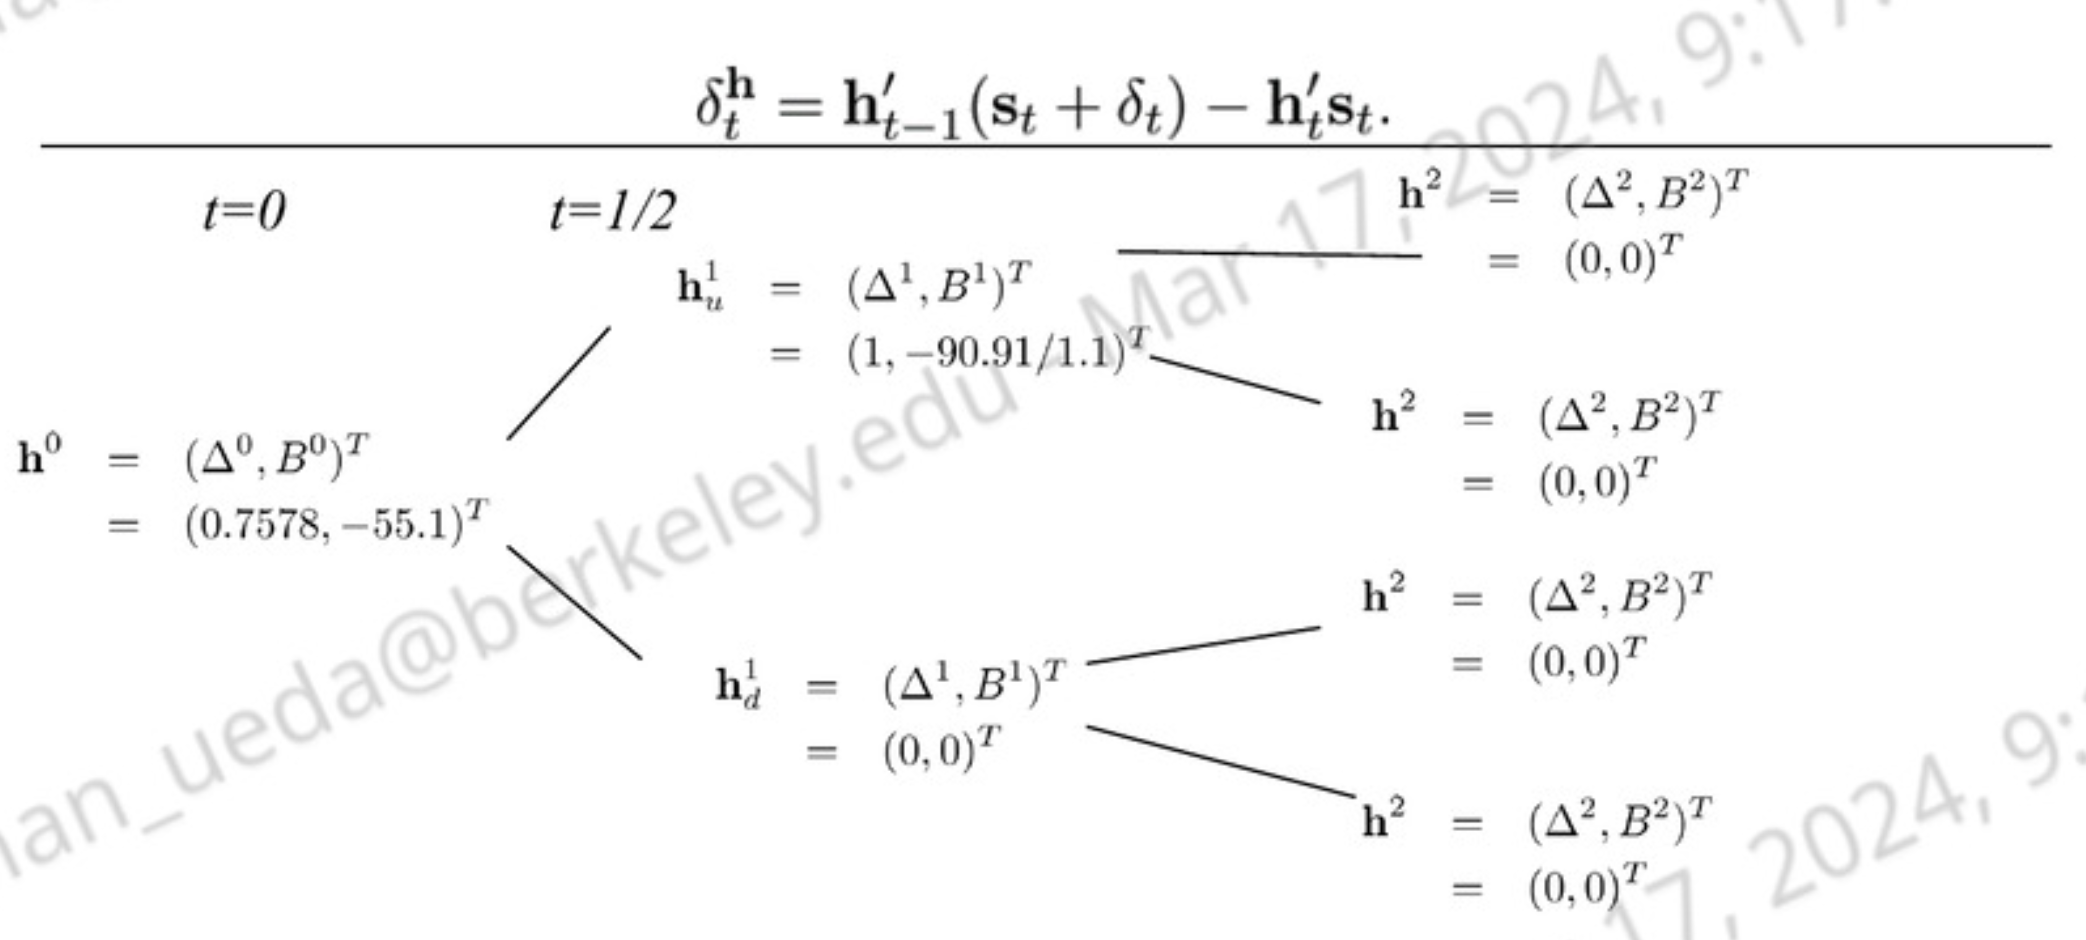
\includegraphics[width=5in]{imgs/multiperiod_security_example.png}
    \caption{Multiperiod security market} 
\end{figure}

By convention 

\[
\boldsymbol{h}_{-1} 
= \begin{bmatrix}
    0 \\
    0
\end{bmatrix}
\]


We can use 
\[
    \delta_t^{\boldsymbol{h}} = \boldsymbol{h}'_{t-1}(\boldsymbol{s}_t + \delta_t) - 
    \boldsymbol{h}'_{t}\boldsymbol{s}_t
\]

Since there are no dividends, we can reduce the equation to 

\[
    \delta_0^{\boldsymbol{h}} = \boldsymbol{h}'_{-1}\boldsymbol{s}_0 - \boldsymbol{h}'_{0}
    \boldsymbol{s}_0
    = \begin{bmatrix}
        0 & 0
    \end{bmatrix}
    \begin{bmatrix} 
        100 \\ 
        1 
    \end{bmatrix} -
    \begin{bmatrix}
        0.7578 & -55.1    
    \end{bmatrix}
    \begin{bmatrix} 
        100 \\ 
        1 
    \end{bmatrix} = -20.67
\]
This states that, to hold $\boldsymbol{h}'_{0} \boldsymbol{s}_0$ at time $t=0$, we need to pay 
$20.67$ at time $t=-1$.

\subsection{Example}
Determine which of the following four processes are adapted w.r.t. to the filtration below.

\begin{figure}[H] 
    \centering 
    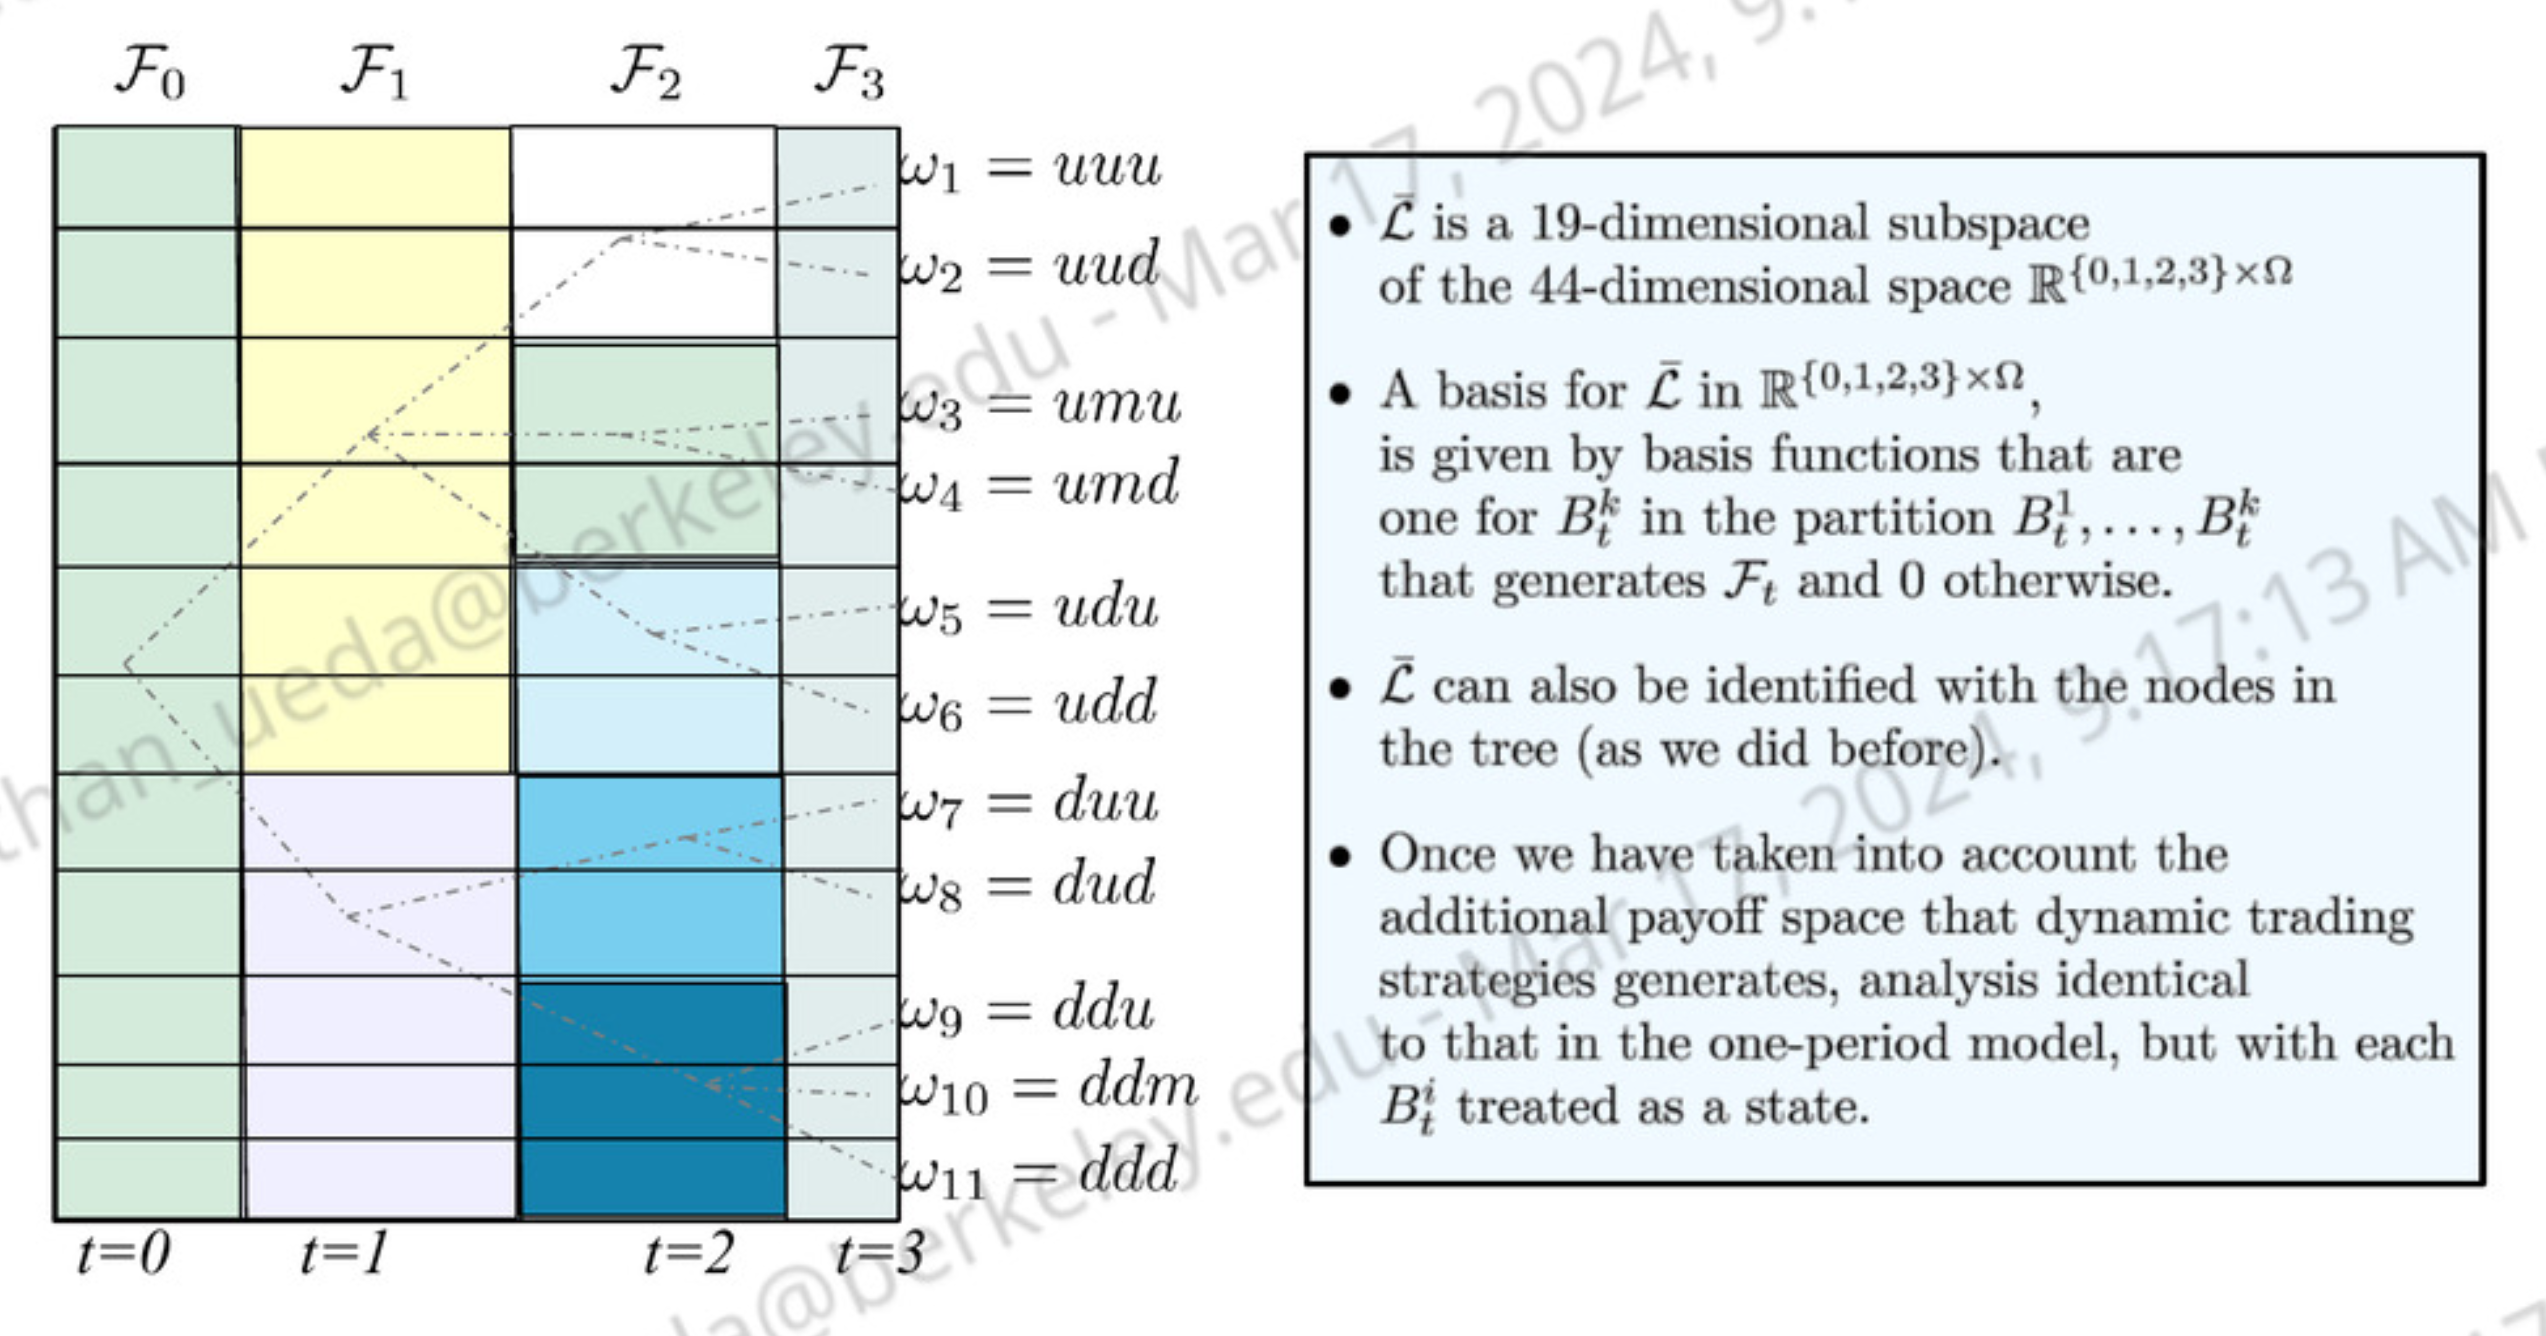
\includegraphics[width=6in]{imgs/embedding.png}
    \caption{The augmented payoff space is 19 dimensional}
\end{figure}


\[f_t : \Omega \rightarrow \mathbb{R}\]
\begin{enumerate}
    \item $f(t, \omega_i) = i + t$ \\ 
    Here, we are at time $t$ in state $\omega_i$. The answer is no and an example to show this 
    is at $t=1$, with states $\omega_1$ and $\omega_2$. Regarding these 2 states, all we know 
    at $t=1$ is they are in the same filtration (i.e. both should evaluate to the same value 
    since they are part of the same filtration). However, upon evaluation we get different 
    values 
    \[f(1, \omega_1) = 1 + 1 = 2 \]
    \[f(1, \omega_2) = 2 + 1 = 3 \]
    \[f(1, \omega_2) \ne f(1, \omega_1) \]


    \item $f(t, \omega_i) = t$ \\ 
    The answer here is yes since it is adaptive. \\
    
    For the next 2 questions, let $\chi$ be an indicator r.v. (has value of 1 or 0 when its 
    corresponding statement is true)
    \item $f(t, \omega_i) = {(t^2 - t)}{\chi_{i \ge 5}}$ \\ 
    The answer here is yes. When $=0$, every state is part of the same filtration which checks 
    out and the same goes for when $t=1$. At $t=2$, the line we can drawn between the 
    indicator r.v. giving us a 1 or a 0 is the line between $\omega_4$ and $\omega_5$ and we 
    notice no blocks are being split up.

    \item $f(t, \omega_i) = {(t^2 - t)}{\chi_{i \ge 6}}$
    The answer here is no. At $t=2$ the line between the indicator r.v. is drawn between 
    $\omega_5$ and $\omega_6$, splitting up two states that should be together at $t=2$.
\end{enumerate}

\section{Continuous Time Models Examples}


\subsection{It\^{o}s Lemma Examples}
\begin{itemize}
    \item Assume $X_t$ is an Ito process that satisfies $dX = u \, dt + v \,dW$, where $W$ is 
    a Brownian motion, and that $Y_t = g(t, X_t)$ for some smooth function $g$. Then $dY_t$ 
    can be written 
    \[dY_t = g_t \,dt + g_x \,dX + \frac{1}{2} g_{xx} {(dX)}^2\]
\end{itemize}



\section{Appendix}
\subsection{Operator Overloading}
For some vector $\boldsymbol{a}$, we write
\begin{itemize}
    \item $\boldsymbol{a} \ge \boldsymbol{0}$ if all elements are nonnegative
    \item $\boldsymbol{a} > \boldsymbol{0}$ if at least one element is strictly positive
    \item $\boldsymbol{a} >> \boldsymbol{0}$ if all elements are strictly positive
\end{itemize}
Similarly,
\begin{itemize}
    \item $\boldsymbol{a} \le \boldsymbol{0}$ if all elements are nonpositive
    \item $\boldsymbol{a} < \boldsymbol{0}$ if at least one element is strictly negative
    \item $\boldsymbol{a} << \boldsymbol{0}$ if all elements are strictly negative
\end{itemize}
\end{document}
